\section{Introduction}
Supervised learning techniques require a large amount of labeled data to train models to classify new data~\cite{jiang_wrapper_2019,jiang_class_2019}. Traditionally, data labeling has been assigned to experts in the domain or well-trained annotators~\cite{tian_MaxMargin_2019}. Although this method produces high-quality labels, it is inefficient and costly~\cite{li_noise_2016,li_noise_2019}.  Social networking provides an innovative solution to the labeling problem by allowing data to be labeled by online crowd annotators. This has become feasible, as crowdsourcing services such as Amazon Mechanical Turk (formerly CrowdFlower) have grown in popularity. Crowdsourcing systems have been used to accumulate large amounts of labeled data for applications such as computer vision~\cite{deng_imagenet_2009,liu_Variational_2012} and natural language processing~\cite{karger_Budget_2014}. However, because of individual differences in preferences and cognitive abilities, the quality of labels acquired by a single crowd annotator is typically low, thus jeopardizing applications that rely on these data. This is because crowd annotators are not necessarily domain experts and may lack the necessary training or expertise to produce high-quality labels.
Aggregation after repeated labeling is one method for handling annotators with various abilities. Label aggregation is a process used to infer an aggregated label for a data instance from a multi-label set~\cite{sheshadri_SQUARE_2013}. Several studies have demonstrated the efficacy of repeated labeling~\cite{tu_multilabel_2018,zhang_multilabelinferencecrowdsourcing_2018}. Repeat labeling is a technique in which the same data are labeled by multiple annotators, and the results are combined to estimate an aggregated label using majority voting (MV) or other techniques. In the case of MV, an aggregated label is the label that receives the most votes from the annotators for a given data instance. This can help reduce the impact of biases or inconsistencies made by annotators. Several factors, such as problem-specific characteristics, the quality of the labels created by the annotators, and the amount of data available, can influence the effectiveness of the aggregation methodologies. Consequently, it is difficult to identify a clear winner among the different techniques. For example, in binary labeling, one study~\cite{sheshadri_SQUARE_2013} discovered that Raykar's~\cite{raykar_Learning_2010} technique outperformed other aggregation techniques. However, according to another study~\cite{zheng_Truth_2017}, the traditional Dawid-Skene (DS) model~\cite{dawid_Maximum_1979} was more reliable in multi-class settings (where data instances can be labeled as belonging to multiple classes).
Furthermore, regardless of the aggregation technique used, the performance of many aggregation techniques in real-world datasets remains unsatisfactory~\cite{liu_Exploiting_2021}. This can be attributed to the complexity of these datasets, which often do not align with the assumptions and limitations of different methods. For example, real-world datasets may present issues such as labeling inaccuracies, class imbalances, or overwhelming sizes that challenge efficient processing with available resources. These factors can adversely affect the effectiveness of label aggregation techniques, potentially yielding less than optimal results for real-world datasets.
Prior information may be used to enhance the label aggregation procedure.
This can include domain knowledge, the use of quality control measures and techniques that account for the unique characteristics of annotators and data. Knowing the reliability of certain annotators, it is possible to draw more accurate conclusions about labels~\cite{li_Crowdsourced_2017}. For instance, in the label aggregation process, labels produced by more reliable annotators (such as domain experts) may be given greater weight. The results of the label aggregation process can also be validated using expert input~\cite{liu_Improving_2017}. During the labeling process, domain experts can provide valuable guidance and oversight to ensure that the labels produced are accurate and consistent.
The agnostic requirement for general-purpose label aggregation is that label aggregation cannot use information outside the labels themselves. This requirement is not satisfied in most label aggregation techniques~\cite{zhang_Crowdsourced_2019}. The agnostic requirement ensures that the label aggregation technique is as general as possible and applicable to a wide range of domains with minimal or no additional context.
The uncertainty of annotators during labeling can provide valuable prior knowledge to determine the appropriate amount of confidence to grant each annotator while still adhering to the requirement of a general-purpose label aggregation technique. We developed a method for estimating the reliability of different annotators based on the annotator's own consistency during labeling. We take this concept a step further by calculating a weight for each annotator based not only on their own reliability but also on the reliability scores of all other workers involved. This consideration of inter-reliability ensures a more comprehensive and dynamic weighting process, adjusting to the overall performance of the entire group of annotators. Thus, the generated weights become a robust measure of both individual and collective trustworthiness, which significantly improves the accuracy and efficacy of our labeling aggregation method.
We propose a novel method called ``crowd-certain'', which provides a more accurate aggregation of labels, ultimately leading to improved overall performance in both crowdsourcing and ensemble learning scenarios. The proposed method uses the consistency of annotators versus a trained classifier to determine their reliability. The experimental results conducted on multiple crowdsourcing datasets show that the proposed techniques generate a weight that closely follows a pre-set ground-truth accuracy, for that each annotator. The proposed techniques outperform prior methods  (Gold Majority Vote, MV, MMSR, Wawa, Zero-Based Skill, GLAD, and Dawid Skene), in terms of accuracy of the aggregated labels with respect to the ground truth labels, particularly when few annotators are available.
The remainder of this paper is organized as follows. Section~\ref{sec:crowd.relatedwork} examines related work involving label aggregation algorithms. In Section~\ref{sec:crowd.method}, we provide a detailed explanation of our proposed technique. Section\ref{sec:crowd.results} presents the experiments and findings. Finally, Section~\ref{sec:crowd.discussion} summarizes the findings and identifies the main directions for future research.

\section{Related Work}\label{sec:crowd.relatedwork}
Numerous label aggregation algorithms have been developed to capture the complexity of crowdsourced labeling systems, including techniques based on annotator reliability~\cite{bi_Learning_2014,demartini_Zencrowd_2012}, confusion matrices~\cite{raykar_Learning_2010,zhang_Spectral_2014}, intentions~\cite{bi_Learning_2014,kurve_MultiCategory_2015}, biases~\cite{zhang_Imbalanced_2013,hernandez-gonzalez_Note_2019, welinder_Multidimensional_2010}, and correlations~\cite{ma_Gradient_2020}. However, because crowdsourced labeling is inherently dynamic and uncertain, developing a technique that can work in most situations is extremely challenging. Many techniques~\cite{liu_Variational_2012,karger_Budget_2014,raykar_Learning_2010,dalvi_Aggregating_2013,ghosh_Who_2011} utilize the Dawid and Skene (DS) generative model~\cite{dawid_Maximum_1979}. Ghosh~\cite{ghosh_Who_2011} extended the DS model by using singular value decomposition (SVD) to calculate the reliability of the annotator. Similarly to Ghosh~\cite{ghosh_Who_2011}, Dalvi~\cite{dalvi_Aggregating_2013} used SVD to estimate true labels with a focus on the sparsity of the labeling matrix. In crowdsourcing, it is common for the labeling matrix to be sparse, meaning that not all annotators have labeled all the data. This may be due to several factors, such as the cost of labeling all data instances or the annotators' time constraints. Karger~\cite{karger_Budget_2014} described an iterative strategy for binary labeling based on a one-coin model~\cite{ghosh_Who_2011}. Karger~\cite{karger_Budget_2014} extends the one-coin model to multi-class labeling by converting the problem into $k-1 $ binary problems (solved iteratively), where $k $ is the number of classes.
The MV technique assumes that all annotators are equally reliable. For segmentation, Warfield~\cite{warfield_Simultaneous_2004} proposed simultaneous truth and performance level estimation (STAPLE), a label fusion method based on expectation maximization. STAPLE ``weighs'' expert opinions during label aggregation by modeling their reliability. Since then, many variants of this technique have been proposed~\cite{winzeck_ISLES_2018,commowick_Objective_2018,asman_Robust_2011,asman_Formulating_2012, eugenioiglesias_Unified_2013, jorgecardoso_STEPS_2013,asman_NonLocal_2013,akhondi-asl_Logarithmic_2014}. The problem with these label aggregation approaches is that they require the computation of a unique set of weights for each sample, necessitating the re-evaluation of the annotators' weights when a new instance is added.
Among the numerous existing label aggregation strategies, MV remains the most efficient and widely used approach~\cite{tao_Label_2020}. If we assume that all annotators are equally reliable and that their errors are independent of one another, then, according to the theory of large numbers, the likelihood that the MV is accurate increases as the number of annotators increases. However, the assumption that all annotators are equally competent and independent may not always hold. Furthermore, MV does not provide any additional information on the degree of disagreement among the annotators (As an example, consider the scenario where four of seven doctors think patient A needs immediate surgery, while all seven think patient B needs immediate surgery; MV will simply label ``yes'' in both cases).
To address this problem, additional measures such as inter-annotator agreement (IAA) have been used~\cite{artstein_InterAnnotator_2017}. IAA is a measurement of the agreement among multiple annotators who label the same data instance. Typically, IAA is calculated using statistical measures, such as Cohen's kappa, Fleiss's kappa, or Krippendorff's alpha~\cite{krippendorff_Content_2018}. These measures consider both the observed agreement between the annotators and the expected agreement owing to random chance. IAA can also be visualized using a confusion matrix or annotation heatmap, which illustrates the distribution of labels assigned by the annotators. This can help identify instances where the annotators disagree or are uncertain and can guide further analysis to improve the annotation~\cite{carletta_Assessing_1996}.
Recently, Sheng~\cite{sheng_Majority_2019} proposed a technique that provided a confidence score along with an aggregated label. The main problem with this approach is that it assumes that all annotators are equally capable when calculating the confidence score. Tao~\cite{tao_Label_2020} improved Sheng's approach by assigning different weights to annotators for each instance. This weighting method combines the specific quality $s_\alpha^{(i,k)} $ for the annotator $\alpha $ and instance $i $ and the overall quality $\tau_\alpha$ across all instances. Inspired by Li's technique~\cite{li_Incorporating_2018}, Tao evaluates the similarity between the annotator labels for each instance. To derive the specific quality $s_{\alpha}^{(i)}$, Tao counts the number of annotators who assigned the same label as the annotator $\alpha $ for that instance. To calculate the overall quality $\tau_\alpha $, Tao performs a 10-fold cross-validation to train each of the 10 classifiers on a different subset of data using the labels provided by the annotator $\alpha $ as true labels and then assigns the average accuracy of the classifiers across all remaining instances as $\tau_\alpha $. The final weight for annotator $\alpha $ and instance $i $ is then calculated using the sigmoid function $\gamma_{i,\alpha}=\tau_\alpha\left(1+{\left(s_{\alpha}^{(i)}\right)}^{2}\right) $. However, Tao's technique~\cite{tao_Label_2020} has some drawbacks. It relies on the labels of other annotators to estimate $s_{\alpha}^{(i)} $. However, different annotators have varying levels of competence (reliability) when labeling the data, and therefore, relying on their labels to measure $s_{\alpha}^{(i)} $ will result in propagating the errors and biases of their labels during weight estimation. Furthermore, Tao's technique~\cite{tao_Label_2020} relies on the labels provided by each annotator $\alpha $ to estimate their respective $\tau_\alpha $ by assuming that the trained classifiers can learn the inherent characteristics of the datasets even in the absence of ground truth labels. While that may be true in some cases, it typically leads to suboptimal measurement and the propagation of biases and errors, from both the annotator's labels and the classifier, into weight estimation.

\section{Methods}\label{sec:crowd.method}
We propose a novel method called ``crowd-certain'' which focuses on leveraging uncertainty measurements to improve decision-making in crowdsourcing and ensemble learning scenarios. Crowd-Certain employs a weighted soft majority voting approach, where the weights are determined based on the uncertainty associated with each annotator's labels. Initially, we use uncertainty measurement techniques to calculate the degree of consistency of each annotator during labeling. Furthermore, to ensure that the proposed technique does not calculate a high weight for annotators who are consistently wrong (for example, when a specific annotator always mislabels a specific class, and hence demonstrates a high consistency even if they label instances incorrectly), we extend the proposed technique by penalizing the annotators for instances in which they disagree with the aggregated label obtained using MV\@. To mitigate the reliance on training a classifier on an annotator's labels, which may be inaccurate, we train an ensemble of classifiers for each annotator. In addition, we report two confidence scores along with the aggregated label to provide additional context for each calculated aggregate label. We report a single weight for all instances in the dataset. As will be demonstrated in Section~\ref{sec:crowd.results}, the proposed crowd-certain method is not only comparable to other techniques in terms of accuracy of the aggregated labels with respect to the ground truth labels for scenarios with a large number of annotators, but also provides a significant improvement in accuracy for scenarios where the number of annotators may be limited. Furthermore, by assigning a single weight to each annotator for all instances in the dataset, the model can assign labels to new test instances without recalculating the annotator weights. This is especially advantageous in situations where annotators are scarce as it enables the model to make accurate predictions with minimal dependence on the annotator input. This characteristic of the crowd-certain method can significantly reduce the time and resources required for labeling in practical applications. When deploying the model in real-world scenarios such as medical diagnosis, fraud detection, or sentiment analysis, it could be advantageous to be able to assign labels to new instances without constantly recalculating annotator weights.
\subsection{Glossary of Symbols}
For convenience, the following list summarizes the major symbols used in the subsequent discussion:
\begin{itemize}[itemsep=1em]
\renewcommand{\textbullet}{}
    \item  $N$: Number of instances.
    \item  $M$: Number of annotators.
    \item  $y^{(i,k)} \in \{0,1\} $: True label for the $k $-th class for instance $i $.
    \item  $z_\alpha^{(i,k)} \in \{0,1\} $: Label given by annotator $\alpha $ for $k $-th class for instance $i $.
    \item  ${{\underset\alpha{\mathrm{MV}}}{\left(z_\alpha^{(i,k)}\right)}} $: Majority voting technique (the label that receives the most votes) applied to annotator labels for class $k $ and instance $i $.
    \item  $\pi_\alpha^{(k)} $: Probability threshold used as pre-set ground truth accuracy, for each annotator $\alpha$ and class $k$. It is used to generate sample binary labels (fictitious ground truth label set) for annotator $\alpha $ for class $k $. For example, the threshold values may be obtained from a uniform distribution in the interval $0.4 $ to $1 $, i.e., $\pi_\alpha^{(k)} \sim U(0.4,1) $.
    \item  $X^{(i)} $: Data for instance $i$.
    \item  $Y^{(i)}=\left\{y^{(i,1)},y^{(i,2)},\;\dots,y^{(i,K)}\right\} $: True label set, for instance $i $. For example, consider a dataset that is labeled for the presence of cats, dogs, and rabbits in any given instance. If a given instance $X^{(i)} $ has cats and dogs but not rabbits, then $Y^{(i)}=\{1,1,0\} $.
    \item  $Z_{\alpha}^{(i)}=\left\{z_\alpha^{(i,1)}, z_\alpha^{(i,2)}, \dots, z_\alpha^{(i,K)}\right\} $: Label set given by the annotator $\alpha $ for instance $i $.
    \item $K$: number of categories (aka classes) in a multi-class multi-label problem. For example, if we have a dataset labeled for the presence of cats, dogs, and rabbits in any given instance, then $K=3$.
    \item  $\rho^{(i)}$: Randomly generated number  between 0 and 1 for instance $i $. It is obtained from a uniform distribution, i.e., $\rho^{(i)} \sim U(0,1) $ This number is used to determine, for each instance $i$, whether the true label should be assigned to each fictitious annotator's label. For each class $k$, if the annotator's probability threshold $\pi_\alpha^{(k)}$ is greater than $\rho^{(i)}$, the true label $y^{(i,k)}$ is assigned; otherwise, an incorrect label $1 - y^{(i,k)}$  is assigned.
    \item  $\Pi_\alpha=\left\{ \pi_\alpha^{(1)} , \pi_\alpha^{(2)}  , \dots, \pi_\alpha^{(K)} \right\} $: set of $K $ probability thresholds for annotator $\alpha $.
    \item  $\mathbb{X}=\left\{X^{(i)}\right\}_{i=1}^{N} $: Set of all instances.
    \item  $\mathbb{Y}=\left\{Y^{(i)}\right\}_{i=1}^{N} $: Set of all true labels.
    \item  $\mathbb{Z}_\alpha=\left\{Z_\alpha^{(i)}\right\}_{i=1}^{N} $: Set of all labels for the annotator $\alpha $.
    \item  $\widehat{\mathbb{Y}}= \left\{\widehat{Y}^{(i)}\right\}_{i=1}^{N} $: Set of all aggregated labels.
    \item  $\mathbb{P}=\left\{\rho^{(i)}\right\}_{i=1}^{N} $: Set of $N $ randomly generated numbers .
    \item  $\mathbb{D}=\left\{\mathbb{X},\mathbb{Y}\right\} $: Dataset containing all instances and all true labels.
    \item  $\mathbb{D}_\alpha=\left\{\mathbb{X},\mathbb{Z}_\alpha\right\} $: Dataset containing the labels given by the annotator $\alpha $.
    \item  $\mathbb{D}_\alpha^\text{train}$, $\mathbb{D}_\alpha^{\text{test}} $: Train and test crowd datasets randomly selected from $\mathbb{D}_{\alpha} $ where $\mathbb{D}_\alpha^{\text{train}} U \mathbb{D}_\alpha^{\text{test}} = \mathbb{D}_\alpha $ and $\mathbb{D}_\alpha^{\text{train}} \bigcap \mathbb{D}_{\alpha}^{\text{test}}=\varnothing $
    \item  $f_{\alpha}^{(g)}(\cdot)$: Classifier $g $ trained on dataset $\mathbb{D}_{\alpha}^{\mathrm{train}} $ with random seed number $g $ (which is also the classifier index)
    \item  $P_{\alpha}^{(i),(g)} = \left\{ p_{\alpha}^{(i,k),(g)} \right\}_{k=1}^{K} $: Predicted probability set obtained in the output of the classifier $f_{\alpha}^{(g)}(\cdot) $ representing the probability that each class $k $ is present in the sample.
    \item  $\theta_{\alpha}^{(k),(g)} $: Binarization threshold. To obtain this, we can utilize any existing thresholding technique. For example, in one technique, we analyze the ROC curve and find the corresponding threshold where the difference between the true positive rate (sensitivity) and false positive rate (1-specificity) is maximum. Alternatively, we could simply use $0.5 $.
    \item  $t_\alpha^{(i,k),(g)} =
        \begin{cases}
            1 & \text{if } p_\alpha^{(i,k),(g)} \geq \theta_\alpha^{(k),(g)}, \\
            0 & \text{otherwise}.
        \end{cases} $: Predicted label obtained by binarizing $p_\alpha^{(i,k),(g)} $.
    \item  $\eta_{\alpha}^{(i,k)} = {{\underset g{\mathrm{MV}}}{ \left(t_\alpha^{(i,k),(g)}\right) }} $: The output of the majority vote applied to the predicted labels obtained by the $G $ classifiers.
    \item  $\Delta_{\alpha}^{(i,k)} $: Uncertainty score.
    \item  $c_\alpha^{(i,k)} $: Consistency score.
    \item  $\omega_\alpha^{(k)} $: Estimated weight for annotator $\alpha $ and class $k $.
    \item  $\nu^{(i,k)} = \frac{1}{{M}}{\sum_{\alpha}{\omega_\alpha^{(k)} \; \eta_\alpha^{(i,k)}}} $ : Final aggregated label for class $k $ and instance $i $.
\end{itemize}
\subsection{Risk Calculation}
Label aggregation is frequently used in various machine learning tasks, such as classification and regression, when multiple annotators assign labels to the same data points. The aggregation model refers to the underlying function that maps a set of multiple labels, obtained by different annotators, into one aggregated label. In the context of label aggregation, this model can be a neural network, a decision tree, or any other machine learning algorithm capable of learning to aggregate labels provided by multiple annotators. The objective of this study is to develop an aggregation model capable of accurately determining true labels despite potential disagreements among annotators. One common method to achieve this involves minimizing the total error (or disagreement) between the annotators' assigned labels and the true labels, as follows:
\begin{equation}
E = \sum_{i=1}^N \sum_{a=1}^M \left( \sum_{k=1}^K \delta\left(y^{(i,k)}, z_\alpha^{(i,k)}\right) \right)
\label{eq:crowd.Eq.1.risk.error}
\end{equation}
where $\delta $ is the Kronecker delta function.
Although error is a crucial aspect in determining the aggregation model's performance, it treats false positives and false negatives with equal weight. However, in many practical scenarios, it is essential to weigh false positives and false negatives differently depending on the specific context and potential consequences of each type of misclassification. The concept of risk allows us to achieve this by incorporating a loss function, which assigns different weights to different types of errors. In this way, risk serves as a weighted calculation of error, enabling us to better evaluate the performance of an aggregation model and its generalization capability.
Let us denote loss function, $\mathcal{L}(\cdot)$, as a function that quantifies the discrepancy between the predicted labels and the true labels, accounting for the varying importance of different types of errors.
Risk, denoted as $R(h) $, represents the expected value of a loss function over all possible data instances.  In practice, our goal is to minimize the risk to achieve optimal performance on unseen data. However, since we only have access to a limited dataset (empirical distribution), we instead work with the empirical risk. This limitation may arise because of the need to reserve a portion of our data for testing and validation or because no dataset can fully capture all possible data instances in the real world. However, minimizing risk alone could result in overfitting, in which the aggregation model learns the noise in the training data rather than the underlying patterns, resulting in poor generalization to unseen data. To improve generalizability, it is necessary to employ regularization techniques to strike a balance between the complexity of the aggregation model and its ability to fit the training data.
Risk measurement enables us to assess the aggregation model's performance in terms of accuracy (of the aggregated labels with respect to the ground truth labels), overfitting (when risk is minimized but the model performs poorly on unseen data), and model complexity.
Assume that the aggregation model $h (\cdot) $ is a function that takes a set of $M $ label sets $Z^{(i)} $ for each instance $i $ in the training data and calculates an aggregated label set $\widehat{Y}^{(i)} $ as an estimate of the true label set $Y^{(i)} $. Our goal is to find an aggregation model $h(\cdot) $ that minimizes risk defined as follows:
\begin{equation}
R(h) = \frac{1}{N} \sum_{i=1}^{N} \mathcal{L} \left( Y^{(i)}, h\left(\left\{Z_{\alpha}^{(i)}\right\}_{\alpha=1}^{M}\right)\right)
\label{eq:crowd.Eq.2.risk.emp}
\end{equation}
In this context, $\mathcal{L}(\cdot) $ represents an arbitrary loss function, which quantifies the discrepancy between predicted labels and true labels while accounting for the varying importance of different types of errors.
Our goal is to choose an aggregation model $\widehat{h} $ that minimizes the risk, following the principle of risk minimization~\cite{vapnik_Principles_1991}:
\begin{equation}
\widehat{h} = \underset{h}{\text{argmin}}  R(h)
\label{eq:crowd.Eq.3.risk.h}
\end{equation}

\subsection{Generating Annotators' Label Sets from Ground Truth}\label{subsec:methods.generating_fictitious_labelset}
In order to evaluate the proposed crowd-certain technique (with and without penalization) as well as other aggregation techniques, we create $M$ fictitious annotators. To synthesize a multi-annotator dataset from a dataset with existing ground truth, we use a uniform distribution in the interval from $0.4 $ to $1 $, i.e., $\pi_\alpha^{(k)} \sim U\left(0.4,1\right) $ (however other ranges can also be used) to obtain $M \times  K$ probability thresholds $\Pi $, where $K$ is the number of classes. (Note that
an annotator may be skilled at labeling dogs, but not rabbits.) Then we use these probability thresholds to generate the crowd label set $Z_{\alpha}^{(i)} $ from the ground truth labels for each instance $i $.
For each annotator $\alpha $, each instance $i $ and class $k $ in the dataset is assigned its true label with probability $\pi_\alpha^{(k)}$ and the opposite label with probability $ (1-\pi_\alpha^{(k)})$. To generate the labels for each annotator $\alpha $, a random number $0 < \rho^{(i)} < 1 $ is generated for each instance $i $ in the dataset. Then $\forall \alpha,k \; \; \text{if} \; \; \rho^{(i)}\leq \pi_\alpha^{(k)}$. Then the true label is used for that instance and class for the annotator $\alpha $; otherwise, the incorrect label is used.
The calculated annotator labels $z_{\alpha}^{(i,k)} $ for each annotator $\alpha $, instance $i $ and class $k $ are as follows:
\begin{equation}
    z_{\alpha}^{(i,k)} =
    \begin{cases}
        y^{(i,k)} & \text{if } \rho^{(i)}  \leq \pi_\alpha^{(k)} , \\
        1 - y^{(i,k)} & \text{if } \rho^{(i)} > \pi_\alpha^{(k)} ,
    \end{cases} \quad \forall i, a, k
    \label{eq:crowd.Eq.4.fictitious_label}
\end{equation}
To evaluate the proposed techniques over all data instances, a k-fold cross-validation is employed.

\subsection{Uncertainty Measurement}\label{subsec:crowd.uncertainty}
A common approach to measure uncertainty is to increase the number of data instances $X $ in the test dataset $\mathbb{D}_\alpha^{\mathrm{test}} $ to create multiple variations of each sample data $X^{(i)} $~\cite{ayhan_TestTime_2018}. In this approach, for each instance $i $, we apply randomly generated spatial transformations and additive noise to the input data $X^{(i)} $ to obtain a transformed sample and repeat this process $G $ times to obtain a set of $G $ transformed samples.
However, this approach is mostly suitable for cases where the input data comprises images or volume slices. Since the datasets used in this study consist of feature vectors instead of images or volume slices, this approach cannot be used. To address this problem, we introduced a modified uncertainty measurement approach, in which instead of augmenting the data instances $X^{(i)} $, we feed the same sample data to different classifiers.
For the choice of classifier, we can either use a probability-based classifier such as random forest and train it under $G $ different random states or train various classifiers and address the problem in a manner similar to ensemble learning~\cite{zhou_Ensemblelearning_2009} (using a set of $G $ different classification techniques such as random forest, SVM, CNN, Adaboost, etc.). In either case, we obtain a set of $G $ classifiers ${\left\{f_{\alpha}^{(g)}( \cdot)\right\}}_{g=1}^G $ for each annotator $\alpha $. The classifier $f_{\alpha}^{(g)}( \cdot) $ is a pre-trained or pre-designed model that has been trained on a labeled training dataset $\mathbb{D}_\alpha^{\mathrm{train}} $. This training process enables $f_{\alpha}^{(g)}(\cdot) $ to learn the underlying patterns in the data and make predictions on unseen instances.
After training, we feed the test samples $X^{(i)}\in \mathbb{X}^{\text{test}} $ to the $g $-th classifier $f_{\alpha}^{(g)}(\cdot) $ as test cases. The classifier $f_{\alpha}^{(g)}(\cdot) $ then outputs a set of predicted probabilities $\left\{p_{\alpha}^{(i,k),(g)}\right\}_{k=1}^{K} $ representing the probability that class $k $ is present in the sample. Consequently, we obtain a collection of $G $ predicted probability sets $\left\{ \left\{ p_{\alpha}^{(i,k),(g)}\right\}_{k=1}^K \right\}_{g=1}^G $ for each annotator $\alpha $ and instance $i $. The set $\left\{p_{\alpha}^{(i,k),(g)}\right\}_{g=1}^G $ contains the predicted probabilities for class $k $, annotator $\alpha $, and instance $i $. Disagreements between predicted probabilities $\left\{p_{\alpha}^{(i,k),(g)}\right\}_{g=1}^G $ can be used to estimate uncertainty.
The reason for using classifiers rather than using the crowdsourced labels directly is two-fold. Using a probabilistic classifier helps us calculate uncertainty based on each annotator's labeling patterns that the classifier learns. Furthermore, this approach provides us with a set of pre-trained classifiers $\left\{ \left\{f_{\alpha}^{(g)}(\cdot) \right\}_{g=1}^G  \right\}_{a=1}^{M} $ that can be readily utilized on any new data instances without the need for those samples to be labeled by the original annotators.
The index value $g  \in \{1,2,\dots,G\} $ is used as the random seed value during training of the $g$\-th classifier for all annotators.
Define $t_{\alpha}^{(i,k),(g)} $ as the predicted label obtained by binarizing the predicted probabilities $p_{\alpha}^{ (i,k),(g)} $ using the threshold $\theta_{\alpha}^{(k),(g)} $ as shown in the Glossary of Symbols section.
Uncertainty measures are used to quantify the level of uncertainty or confidence associated with the predictions of a model. In this work, we need to measure the uncertainty $u_{\alpha}^{(i,k)}$ associated with the model predictions. Some common uncertainty measurement measures are as follows.

\subsubsection{Entropy}
Entropy is a widely used measure of uncertainty in classification problems. In an ensemble of classifiers, entropy serves as a quantitative measure of the uncertainty or disorder present in the probability distribution of the predicted class labels. A higher entropy value indicates a greater degree of uncertainty in the predictions, as the predictions of the individual classifiers in the ensemble are significantly different. In contrast, a lower entropy value indicates reduced uncertainty as the ensemble assigns very similar probabilities to a particular class, indicating strong agreement among the classifiers and increased confidence in their collective prediction. The formula for calculating entropy is as follows:
\begin{equation}
\Delta_{\alpha}^{(i,k)}=H\left(\left\{p_{\alpha}^{(i,k),(g)}\right\}_{g=1}^{G}\right)=-\sum_{g}{p_{\alpha}^{(i,k),(g)} \log\left(p_{\alpha}^{(i,k),(g)}\right)}
\label{eq:crowd.Eq.5.uncertainty}
\end{equation}

\subsubsection{Standard Deviation}
In regression problems, standard deviation is often used to quantify uncertainty. It measures the dispersion of predicted values around the mean. A greater standard deviation indicates greater uncertainty of the prediction. For a set of predicted values $ \{t_{\alpha}^{(i,k),(g)} \}_{g=1}^G $ with mean value $\mu $, the standard deviation is defined as.
\begin{equation}
   \Delta_{\alpha}^{(i,k)}=\text{SD}\left(\left\{t_{\alpha}^{(i,k),(g)}\right\}_{g=1}^G\right)=\sqrt {\frac{1}{G-1 }\sum_{g=1}^G\left(t_{\alpha}^{(i,k),(g)}-\mu\right)^{2}},\quad\mu=\frac{1}{G}\sum_{g=1}^{G}{t_{\alpha}^{(i,k),(g)}}
    \label{eq:crowd.Eq.6.uncertainty.sd}
\end{equation}

\paragraph{Predictive Interval}
A predictive interval provides a range within which a future observation is likely to fall with a certain level of confidence. For example, a 95\% predictive interval indicates that there is a 95\% likelihood that the true value falls within that range. A greater uncertainty corresponds to wider intervals. In the context of multiple classifiers, the predictive intervals can be calculated by considering the quantiles of the classifier output. For a predefined confidence level $\gamma $ (e.g., 95\%), for a specific class $k $, we need to find the quantiles $Q_{L}^{k} $ and $Q_{U}^{k} $ of the probability distribution of class $k $ predicted by the $G $ classifiers. The uncertainty can be represented by the width of the predictive interval:
\begin{equation}
    \begin{aligned}
        P\left(Q_L^{k} \leq p_{\alpha}^{(i,k),(g)} \leq Q_U^{k}\right) = \gamma
        \\
        \Delta_{\alpha}^{(i,k)} = Q_L^{k} - Q_U^{k}
    \end{aligned}
    \label{eq:crowd.Eq.uncertainty}
\end{equation}
The steps to calculate the predictive interval are as follows:
\begin{enumerate}
    \item Collect the class $k $ probabilities predicted by all $G$ classifiers for a given instance. Then sort the values in ascending order. Let us call this set $P_{\alpha}^{(i,k)}=\mathrm{sorted}\left(\left\{p_{\alpha}^{(i,k),(g)}\right\}_{g=1}^G\right),\quad\forall \alpha,k,i $.
    \item Calculate the lower and upper quantile indices based on the chosen confidence level $\gamma $. The lower quantile index is $L=\mathrm{ceil}\left(\frac{G}{2}\left(1-\gamma\right)\right) $, and the upper quantile index is $U=\mathrm{floor}\left(\frac{G}{2} (1+\gamma)\right) $, where ceil and floor are the ceiling and floor functions, respectively.
    \item Find the values corresponding to the lower and upper quantile indices in the sorted $P_{\alpha}^{(i,k)} $. These values are the lower and upper quantiles $Q_L^{k} $ and $Q_U^{k} $.
    \item Now we have the predictive interval $P\left(Q_L^{k}<=p_{\alpha}^{(i,k),(g)}<=Q_U^{k}\right)=\gamma $, where $Q_L^{k} $ and $Q_U^{k} $ represent the bounds of the interval containing the $\alpha$ proportion of the probability mass.
\end{enumerate}
\subsubsection{Monte Carlo Dropout}
The Monte Carlo dropout~\cite{gal_Dropout_2016a} can be used to estimate uncertainty in neural networks by applying the dropout at test time. Multiple forward passes with dropout generate a distribution of predictions from which uncertainty can be derived using any of the aforementioned techniques (standard deviation, entropy, etc.).
\subsubsection{Bayesian Approaches}
Bayesian methods offer a probabilistic framework to estimate the parameters of the model and make predictions. These methods explicitly model uncertainty by considering prior beliefs about the model parameters and then updating those beliefs based on the observed data. In Bayesian modeling, the model parameters are treated as random variables and a posterior distribution is estimated using these parameters. The following are two common Bayesian approaches for measuring the uncertainty in classification problems.
\begin{itemize}
    \item \relax \textbf{Bayesian model averaging (BMA):} BMA accounts for model uncertainty by combining the predictions of various models using their posterior probabilities as weighting factors. Instead of selecting a single ``best'' model, BMA acknowledges the possibility of multiple plausible models, each with its own strengths and weaknesses~\cite{hoeting_Bayesian_1999}. The steps to implement BMA are as follows. Select a set of candidate models that represent different hypotheses regarding the data-generating process underlying the data. These models may be of various types, such as linear regression, decision trees, neural networks, or any other model suited to the specific problem at hand. Using the available data, train each candidate model. Calculate the posterior probabilities of the models. Using the posterior probabilities of each model as weights, calculate the weighted average of each model's predictions. The weighted average is the BMA prediction for the input instance and class.
    \item \relax \textbf{Bayesian neural networks (BNNs):} BNNs~\cite{mullachery_Bayesian_2018} are an extension of conventional neural networks in which the weights and biases of the network are treated as random variables. The primary distinction between BNNs and conventional neural networks is that BNNs model uncertainty directly in the weights and biases. The posterior distributions of the network weights and biases (learned during training) capture the uncertainty, which can then be utilized to generate predictive distributions for each class. This enables multiple predictions to be generated by sampling these predictive distributions, which can be used to quantify the uncertainty associated with each class.
\end{itemize}
\subsubsection{Committee-Based Methods}
The committee-based method~\cite{wang_Wisdom_2020} involves training multiple models (a committee) and aggregating their predictions. The disagreement between committee members' predictions can be used as a measure of uncertainty. Examples include bagging and boosting ensemble methods and models, such as random forests.
\begin{equation}
    \Delta_{\alpha}^{(i,k)} = \mathrm{VarCommittee}\left(P_{\alpha}^{(i,k)}\right) = \frac{1}{G-1}\sum_{g=1}^G \left(p_{\alpha}^{(i,k),(g)}-\mu\right)^{2},\quad\mu= \frac{1}{G} \sum_{g=1}^G p_{\alpha}^{(i,k),(g)}
    \label{eq:crowd.Eq.8.uncertainty.committee_based}
\end{equation}
\subsubsection{Conformal Prediction}
Conformal prediction~\cite{angelopoulos_Gentle_2021} is a method of constructing prediction regions that maintain a predefined level of confidence. These regions can be used to quantify the uncertainty associated with the prediction of a model.
Steps  to calculate the nonconformity score:
\begin{enumerate}
    \item For each classifier $g $ and each class $k $, calculate the nonconformity score. Here, $\mathrm{score\_function}$ measures the conformity of the prediction with the true label. In the context of this study, the true label can be replaced by $\eta_{\alpha}^{(i,k)} $. A common choice for $\mathrm{score\_function}$ is the absolute difference between the predicted probability and the true label, but other options can be used depending on the specific problem and requirements. Define the nonconformity score as $ \zeta_{k}^{g} = \mathrm{score\_function} \left(p_{\alpha}^{(i,k),(g)}, y^{(i,k)}\right) $
    \item Calculate the p-value for each class $k $ as the proportion of classifiers with nonconformity scores greater than or equal to a predefined threshold $\text{T}^{(k)}: \text{p-values}(k) = \frac{ \left\vert \{g: \;\zeta^{(k),(g)} \geq \text{T}^{(k)} \} \right\vert} {G} $
    \item The p-values calculated for each class $k $ represent the uncertainty associated with that class. A higher p-value indicates a higher level of agreement among the classifiers for a given class, whereas a lower p-value suggests greater uncertainty or disagreement.
\end{enumerate}
The uncertainty measures discussed above are only some of the available options. Selecting an appropriate measure depends on factors such as the problem domain, the chosen model, and the specific requirements of a given application. For this study, we use the variance technique shown in Equation~(\ref{eq:crowd.Eq.6.uncertainty.sd}) as our uncertainty measurement due to its simplicity. However, other measures could also be employed as suitable alternatives.
\subsection{Crowd-Certain: Uncertainty-Based Weighted Soft Majority Voting}
\subsubsection{Consistency Measurement}
Define $c_{\alpha}^{(i,k)} $ as the consistency score for annotator $\alpha $, class $k $ and instance $i $. We calculate this consistency score using the uncertainty score $\Delta_{\alpha}^{(i,k)} $ explained in the previous section. We use two approaches to calculate $c_{\alpha}^{(i,k)} $ from $\Delta_{\alpha}^{(i,k)} $.
\begin{enumerate}
    \item The first approach is to simply subtract the uncertainty from $1 $ as follows:
    \begin{equation}
        c_{\alpha}^{(i,k)}=1-\Delta_{\alpha}^{(i,k)}\;\;,\;\forall i,\alpha,k
        \label{eq:crowd.Eq.9.consistency}
    \end{equation}
    \item In a second approach (shown in Equation~(\ref{eq:crowd.eq.10.consistency-penalized})), we penalize annotators for instances in which their predicted label $\eta_{\alpha}^{(i,k)} $ (explained in the Glossary of Symbols section) does not match the MV of all annotator labels ${{\underset \alpha{\mathrm{MV}}}{\left(z_{\alpha,\;k}^{(i,k)}\right)}} $. As previously discussed, instead of directly working with the annotator's labels $z_{\alpha}^{(i,k)} $, we use the predicted labels obtained from the ensemble of classifiers $\eta_{\alpha}^{(i,k)} $. This methodology does not require repeating the crowd-labeling process for new data samples. In particular, we are likely not to have access to the same crowd of annotators employed in the training dataset.
    \begin{equation}
        c_{\alpha}^{(i,k)} =
        \begin{cases}
            1 - \Delta_{\alpha}^{(i,k)} & \text{if } \eta_{\alpha}^{(i,k)} = \operatorname{MV}_{\alpha}(\eta_{\alpha}^{(i,k)}) \\
            0 & \text{otherwise}
        \end{cases}
        \label{eq:crowd.eq.10.consistency-penalized}
    \end{equation}
\end{enumerate}
\subsubsection{Reliability Measurement}
For each annotator, for each class, and for each instance, there is a consistency score, $c_{\alpha}^{(i,k)}$. By averaging these scores across all instances, we can define a reliability score for each annotator and for each class:
\begin{equation}
\psi_{\alpha}^{(k)}=\frac{1}{N}\sum_{i=1}^N c_{\alpha}^{(i,k)}
\end{equation}
If desired, one may also calculate an overall reliability score for each annotator by averaging across all classes:
\begin{equation}
\psi_{\alpha}=\frac{1}{K}\sum_{k=1}^K \psi_{\alpha}^{(k)}
\end{equation}

\subsubsection{Weight Measurement}
Furthermore, we calculate the annotators' weights $\omega_\alpha^{(k)}$ for each class k by normalizing the reliability values as follows:
\begin{equation}
    \omega_{\alpha}^{(k)}=\frac{\psi_{\alpha}^{(k)}}{\sum_{\alpha=1}^{M} \psi_{\alpha}^{(k)}}
    \label{eq:crowd.eq.11.weights}
\end{equation}

\subsubsection{Aggregated Label Calculation}
Finally, the aggregated label $\nu^{(i,k)}$ for each instance $i $ and class $k $ is the weighted average of the predicted labels $\eta_{\alpha}^{(i,k)} $ for each annotator $\alpha $:
\begin{equation}
    \nu^{(i,k)} =
    \begin{cases}
        1 & \text{if } \left(\sum_{\alpha=1}^{M} \omega_{\alpha}^{(k)}\, \eta_{\alpha}^{(i,k)}\right) > 0.5 \\
        0 & \text{otherwise}
    \end{cases}
    \quad \forall i, k
    \label{eq:crowd.Eq.12.aggregated-label}
\end{equation}

\subsubsection{Confidence Score Calculation}
In previous section we showed how to calculate the aggregated label $\nu^{(i,k)}$ (shown in Equation~(\ref{eq:crowd.Eq.12.aggregated-label})). Define $F^{(i,k)} $ as the confidence score for instance $i $ and class $k $. We calculate two confidence scores $F^{(i,k)} $, based on how many different annotators agree on the reported label $\nu^{(i,k)}$. The confidence scores show the level of confidence we should place on the aggregated labels. To calculate this confidence score, we modify the two techniques used by Sheng~\cite{sheng_Majority_2019} and Tao~\cite{tao_Label_2020} to incorporate our calculated weight $\omega_{\alpha}^{(k)} $ shown in Equation~(\ref{eq:crowd.eq.11.weights})  for each worker $\alpha $.

\textbf{Using Weighted Sum:}
In a standard voting system, for every instance $i$ and class $k$, each contributor in the group—whether that be an annotator in a crowd or a model in an ensemble learning context—provides a class label. The label receiving the most votes, meaning it's predicted by the majority of contributors, is selected as the final prediction. This approach is often referred to as majority voting or hard voting.

This method could be improved by taking into account not only the number of votes each label receives, but also the confidence associated with each vote. This factor introduces the notion of a ``weighted sum of all votes for a particular class''. As part of this study, we propose techniques that assign a weight to each contributor in the group. This calculation is based on their voting consistency and the degree to which they concur with their peers.

To compute the weighted sum of all votes for each class, we can combine the calculated weights with the corresponding labels, whether provided or predicted. This calculation gives greater weight to votes with greater confidence, or, in other words, votes with greater weight. This refined approach prioritizes confidence, thereby enhancing the ensemble's overall effectiveness.

The confidence score $F_{\Omega}^{(i,k)}$ is formulated as follow.
\begin{equation}
    F_{\Omega}^{(i,k)} = {\sum\nolimits_{\alpha=1}^{M}{\omega_{\alpha}^{(k)} \delta\left(\eta_{\alpha}^{(i,k)} \;,\;\; \nu^{(i,k)} \right)}}
    \label{eq:crowd.Eq.13.confidence-score.freq}
\end{equation}
where $\delta $ is the Kronecker delta function.


\textbf{Using CDF of beta distribution function:}
The binomial distribution survival function, also referred to as the complementary cumulative distribution function (CCDF), provides the probability of observing a result as extreme or more extreme than a given value. It provides the probability that a random variable drawn from the binomial distribution is greater than or equal to a given value.

It can be applied in the following ways when calculating confidence scores:

\begin{enumerate}
    \item \textbf{Hypothesis testing:}
    Suppose you are testing a hypothesis concerning a parameter of a population, and you collect a sample of observations. Given the null hypothesis, the binomial survival function can be used to calculate the probability of observing a result as extreme or more extreme than the one observed. This probability is the p-value, and if it is very small, the null hypothesis may be rejected. In this context, the confidence score could be interpreted as (1 $-$ p-value), a measure of the certainty with which the null hypothesis can be rejected.

    \item \textbf{Binary classification:} Consider a binary classification problem in which an algorithm sorts objects into two groups, A and B. Given the observed results, the binomial survival function can be used to calculate the probability of misclassification. The confidence score in this instance could be interpreted as (1 $-$ probability of misclassification).
\end{enumerate}

In the following equation, the probability of obtaining k successes or more out of n trials where the probability of success on any given trial is p is calculated. In this context, ``success'' could refer to the event in question, such as the correct classification of an object or the acceptance of a hypothesis. The CDF of the beta distribution at the decision threshold of $0.5 $ is used to calculate a confidence score $F_{\beta}^{(i,k)}$. To calculate the two shape parameters of the beta distributions $l^{(i,k)}$ and $u^{(i,k)}$, a weighted sum of all correct and incorrect aggregated labels, is used respectively:
\begin{equation}
    \begin{aligned}
        l^{(i,k)} &= 1 + \sum_{\alpha=1}^{M} \omega_{\alpha}^{(k)} \; \delta\left(\eta_{\alpha}^{(i,k)}, \nu_{k}^{(i,k)}\right) \\
        u^{(i,k)} &= 1 + \sum_{\alpha=1}^{M} \omega_{\alpha}^{(k)} \; \delta\left(\eta_{\alpha}^{(i,k)}, 1 - \nu_{k}^{(i,k)}\right)
    \end{aligned}
    \label{eq:crowd.Eq.14.beta_l_u}
\end{equation}
%
\begin{equation}
    F_{\beta}^{(i,k)} =I_{0.5}\left(l^{(i,k)},u^{(i,k)}\right)=\sum_{t=[l^{(i,k)}]}^{T-1}\frac{(T-1)!}{t!(T-1-t)!}0.5^{T-1}
    \label{eq:crowd.Eq.15.confidence-score.beta}
\end{equation}
where $T = \left [ l^{(i,k)} + u^{(i,k)} \right >] $ and $\left [ \cdot \right ] $ is an integer function.


\subsection{Metrics}
%
\begin{itemize}
\item \textbf{Accuracy} is defined as follows.
\begin{equation}
    \text{Accuracy}=\delta \left(\nu^{(i,k)}, y^{(i,k)} \right)
\end{equation}
where the $y^{(i,k)}$ and $\nu^{(i,k)}$ are the ground truth and aggregated label respectively for class $k$ and instance $i$.
%
\item \textbf{Calibration:} Calibration measures whether the predicted confidence scores match the actual accuracy of the predictions. In a perfectly calibrated system, if you take all instances where the model assigned a confidence score of 80\%, for example, then about 80\% of those predictions should be correct. A model can be deemed as well-calibrated if the predicted probabilities match the empirical (observed) probabilities. Calibration plots can be a useful tool to visually inspect the calibration of your model. A perfectly calibrated model would have a plot where the points lie on the 45-degree line (y = x).
%
\item \textbf{Brier Score:} The Brier score is a proper score rule that measures the accuracy of probabilistic predictions. It is applicable to tasks of binary and categorical outcomes and can also be used for multilabel tasks with some adaptations. It's calculated as the mean squared difference between the predicted probability and the actual outcome (0 or 1), and thus rewards both good calibration and sharpness (high confidence in correct predictions).
%
\item \textbf{Area Under the ROC Curve (AUC-ROC):} While ROC-AUC is often used to evaluate classification performance, it can also provide an indication of how well the model's confidence in its predictions corresponds with its accuracy. This would involve treating the confidence score as a ranking over the instances, and the true labels as the thing to predict. This works well if higher confidence in a label is supposed to mean that the label is more likely to be correct.
%
\item \textbf{Expected Calibration Error (ECE):} ECE quantifies the calibration of a model. It is computed as a weighted average of the absolute difference between accuracy and confidence in each bin when predictions are grouped into bins based on their predicted confidence.
\end{itemize}

\section{Results}\label{sec:crowd.results}
To evaluate our proposed technique, we conducted a series of experiments comparing the proposed technique with several existing techniques such as MV, Tao~\cite{tao_Label_2020}, and Sheng~\cite{sheng_Majority_2019}, as well as with other crowdsourcing methodologies reported in the crowd-kit package~\cite{ustalov_learning_2021 } including Gold Majority Voting, MMSR~\cite{ma_Adversarial_2020}, Wawa, Zero-Based Skill, GLAD~\cite{whitehill_Whose_2009}, and Dawid Skene~\cite{dawid_Maximum_1979}.

\subsection{Datasets}\label{subsec:results.datasets}
We report the performance of our proposed techniques on various datasets. These datasets cover a wide range of domains and have varying characteristics in terms of the number of features, samples, and class distributions. Table~\ref{tab:crowd.Table.1.Datasets} provides an overview of the datasets used. All datasets are obtained from the University of California, Irvine (UCI) repository~\cite{duan_UCI_2017}.
\begin{table}[!htbp]
\centering
\caption{Descriptions of the datasets used.}
\def\arraystretch{1}
\begin{tabulary}{\linewidth}{LCCCC}
    \toprule
    \textbf{Dataset} & \textbf{\#Features} & \textbf{\#Samples} & \textbf{\#Positives} & \textbf{\#Negatives} \\
    kr-vs-kp    & 36 & 3196 & 1669 & 1527 \\
    mushroom    & 22 & 8124 & 4208 & 3916 \\
    iris        & 4  & 100  & 50   & 50   \\
    spambase    & 58 & 4601 & 1813 & 2788 \\
    tic-tac-toe & 10 & 958  & 332  & 626  \\
    sick        & 30 & 3772 & 231  & 3541 \\
    waveform    & 41 & 5000 & 1692 & 3308 \\
    car         & 6  & 1728 & 518  & 1210 \\
    vote        & 16 & 435  & 267  & 168  \\
    ionosphere  & 34 & 351  & 126  & 225  \\
    \bottomrule
\end{tabulary}%
\label{tab:crowd.Table.1.Datasets}
\end{table}
%
\begin{itemize}
    \item The \textbf{kr-vs-kp} dataset represents the King Rook-King Pawn on a7 in chess. The positive class indicates a victory for white (1,669 instances, or 52\%), while the negative class indicates a defeat for white (1,527 instances, 48\%).
    \item The \textbf{mushroom} dataset is based on the Audubon Society Field Guide for North American Mushrooms (1981) and includes 21 attributes related to mushroom characteristics such as cap shape, surface, odor, and ring type.
    \item The \textbf{Iris} Plants Dataset comprises three classes, each with 50 instances, representing different iris plant species. The dataset contains four numerical attributes in centimeters: sepal length, sepal width, petal length, and petal width.
    \item The \textbf{Spambase} dataset consists of 57 attributes, each representing the frequency of a term appearing in an email, such as the ``address’’.
    \item The \textbf{tic-tac-toe} endgame dataset encodes all possible board configurations for the game, with ``x'' playing first. It contains attributes (X, O, and blank) corresponding to each of the nine tic-tac-toe squares.
    \item The \textbf{Sick} dataset includes thyroid disease records from the Garvan Institute and J. Ross Quinlan of the New South Wales Institute in Sydney, Australia. 3,772 instances with 30 attributes (seven continuous and 23 discrete) and 5.4\% missing data. Attributes include age, pregnancy, TSH, T3, TT4, etc.
    \item The \textbf{waveform} dataset generator comprises 41 attributes and three wave types, with each class consisting of two ``base'' waves.
    \item The \textbf{Car} Evaluation Dataset rates cars on price, buying, maintenance, comfort, doors, capacity, luggage, boot size, and safety using a simple hierarchical decision model. The dataset consists of 1,728 instances categorized as unacceptable, acceptable, good, and very good.
    \item The 1984 US Congressional \textbf{Voting} Records Dataset shows how members voted on 16 CQA-identified critical votes. Votes are divided into nine categories, simplified to yea, nay, or unknown disposition. The dataset has two classes: Democrats (267) and Republicans (168).
    \item The Johns Hopkins \textbf{Ionosphere} dataset contains data collected near Goose Bay, Labrador, using a phased array of 16 high-frequency antennas. ``Good'' radar returns show ionosphere structure, while ``bad'' returns are ionosphere-free. The dataset includes 351 instances with 34 attributes categorized as good or bad.
\end{itemize}

All datasets were transformed into a two-class binary problem for comparison with existing benchmarks. For instance, only the first and second classes were used in the ``waveform'' dataset, and the first two classes were utilized in the ``Iris'' dataset.
We generated multiple fictitious label sets for each dataset to simulate the crowdsourcing concept of collecting several crowd labels for each instance. We selected random samples in the datasets using a uniform distribution and altered their corresponding true labels to incorrect ones, while maintaining the original distribution of the ground-truth labels. The probability of each instance containing the correct true label was determined using a uniform distribution, allowing us to create synthetic label sets for each annotator that preserved the underlying structure and difficulty of the original classification problem. By creating datasets with various levels of accuracy, we can evaluate the performance of the proposed method under different conditions of annotator expertise and reliability. This allows us to assess the ability of our method to handle diverse real-world crowdsourcing scenarios and gain insight into its general applicability and effectiveness in improving overall classification accuracy.

\subsection{Benchmarks}
Tao~\cite{tao_Label_2020} and Sheng~\cite{sheng_Majority_2019} techniques were implemented in Python to evaluate their performance. Furthermore, the crowd-kit package (A General-Purpose Crowdsourcing Computational Quality Control Toolkit for Python)~\cite{ustalov_learning_2021 } was used to implement the remaining benchmark techniques, including Gold Majority Voting, MMSR~\cite{ma_Adversarial_2020}, Wawa, Zero-Based Skill, GLAD~\cite{whitehill_Whose_2009}, and Dawid Skene~\cite{dawid_Maximum_1979}.
%
\begin{itemize}
    \item \textbf{Golden majority voting} estimates the probability that each annotator possesses the correct label and then calculates the probability of each label per occurrence based on the weight assigned to each label. Assume that 10,000 jobs are performed by 3,000 annotators as well as 100 instances of ground truth. First, the percentage of correct labels for each annotator is calculated. The remaining labels are then estimated based on the weights.
    \item \textbf{Worker Agreement with Aggregate (WAWA)~\cite{crowdkit_wawa_2023}:} (Annotator Agreement with Aggregate), also referred to as ``inter-rater agreement'', is a commonly used statistic for non-testing problems. This indicates the average frequency with which each annotator's response matches the aggregate response for each instance.
    \item \textbf{Zero-Based-Skill (ZBS)} employs a weighted majority vote (WMV). After processing a collection of instances, it re-evaluates the abilities of the annotators based on the accuracy of their responses. This process is repeated until the labels no longer change or the maximum number of iterations is reached.
    \item Descriptions of the other techniques can be found in their respective references.
    \item \textbf{Karger-Oh-Shah (KOS):}
        Iterative algorithm that calculates the log-likelihood of the task being positive while modeling
        the reliabilities of the workers.

        Let $A_{ij}$ be a matrix of answers of worker $j$ on task $i$.
        $A_{ij} = 0$ if worker $j$ didn't answer the task $i$, otherwise $|A_{ij}| = 1$.
        The algorithm operates on real-valued task messages $x_{i \rightarrow j}$  and
        worker messages $y_{j \rightarrow i}$. A task message $x_{i \rightarrow j}$ represents
        the log-likelihood of task $i$ being a positive task, and a worker message $y_{j \rightarrow i}$ represents
        how reliable worker $j$ is.

        On iteration $k$ the values are updated as follows:
        \begin{equation}
        x_{i \rightarrow j}^{(k)} = \sum_{j^{'} \in \partial i \backslash j} A_{ij^{'}} y_{j^{'} \rightarrow i}^{(k-1)} \\
        y_{j \rightarrow i}^{(k)} = \sum_{i^{'} \in \partial j \backslash i} A_{i^{'}j} x_{i^{'} \rightarrow j}^{(k-1)}
        \end{equation}
    \item \textbf{Multi-Annotator Competence Estimation (MACE)~\cite{hovy_MACE_2013}:}
            Probabilistic model that associates each worker with a probability distribution over the labels. For each task, a worker might be in a spamming or not spamming state. If the worker is not spamming, they yield a correct label. If the worker is spamming, they answer according to their probability distribution. Let's assume that the correct label $T_i$ comes from a discrete uniform distribution. When a worker annotates the task, they are in the spamming state with probability $\operatorname{Bernoulli}(1 - \theta_w)$. So, if their state $s_w = 0$, their response $A_{iw} = T_i$. Otherwise, their response $A_{iw}$ is drawn from a multinomial distribution with parameters $\xi_w$.
    \item \textbf{Matrix Mean-Subsequence-Reduced Algorithm (MMSR)~\cite{ma_Adversarial_2020}:}
            The M-MSR assumes that workers have different level of expertise and associated            with a vector of ``skills'' $\boldsymbol{s}$ which entries $s_i$ show the probability of the worker $i$ to answer correctly to the given task. Having that, we can show that.
            \begin{equation}
                \mathbb{E}\left[\frac{M}{M-1}\widetilde{C}-\frac{1}{M-1}\boldsymbol{1}\boldsymbol{1}^T\right]
                = \boldsymbol{s}\boldsymbol{s}^T,
            \end{equation}
            where $M$ is the total number of classes, $\widetilde{C}$ is a covariation matrix between
            workers, and $\boldsymbol{1}\boldsymbol{1}^T$ is the all-ones matrix which has the same
            size as $\widetilde{C}$.

            So, the problem of recovering the skills vector $\boldsymbol{s}$ becomes equivalent to the
            rank-one matrix completion problem. The M-MSR algorithm is an iterative algorithm for *rubust* rank-one matrix completion, so its result is an estimator of the vector $\boldsymbol{s}$.
            Then, the aggregation is the weighted majority vote with weights equal to
            $\log \frac{(M-1)s_i}{1-s_i}$.
    %
    \item \textbf{Generative model of Labels, Abilities, and Difficulties (GLAD)~\cite{whitehill_Whose_2009}:}
    A probabilistic model that parametrizes workers' abilities and tasks' dificulties.
    Let's consider a case of $K$ class classification. Let $p$ be a vector of prior class probabilities, $\alpha_i \in (-\infty, +\infty)$ be a worker's ability parameter, $\beta_j \in (0, +\infty)$ be an inverse task's difficulty, $z_j$ be a latent variable representing the true task's label, and $y^i_j$ be a worker's response that we observe. The relationships between this variables and parameters according to GLAD are represented by the following latent label model:
    The prior probability of $z_j$ being equal to $c$ is $\operatorname{Pr}(z_j = c) = p[c],$
    the probability distribution of the worker's responses conditioned by the true label value $c$ follows the single coin Dawid-Skene model where the true label probability is a sigmoid function of the product of worker's ability and inverse task's difficulty:
    \begin{equation}
    \operatorname{Pr}(y^i_j = k | z_j = c) = \begin{cases}a(i, j), & k = c \\ \frac{1 - a(i,j)}{K-1}, & k \neq c\end{cases},
    \end{equation}
    where $a(i,j) = \frac{1}{1 + \exp(-\alpha_i\beta_j)}.$

    Parameters $p$, $\alpha$, $\beta$ and latent variables $z$ are optimized through the Expectation-Minimization algorithm.
    %
    \item \textbf{Dawid-Skene~\cite{dawid_Maximum_1979}:}
    Probabilistic model that parametrizes workers' level of expertise through confusion matrices.   Let $e^w$ be a worker's confusion (error) matrix of size $K \times K$ in case of $K$ class classification, $p$ be a vector of prior classes probabilities, $z_j$ be a true task's label, and $y^w_j$ be a worker's answer for the task $j$. The relationships between these parameters are represented by the following latent label model.
    Here the prior true label probability is $\operatorname{Pr}(z_j = c) = p[c]$ and the distribution on the worker's responses given the true label $c$ is represented by the
    corresponding column of the error matrix: $\operatorname{Pr}(y_j^w = k | z_j = c) = e^w[k, c]$
    Parameters $p$ and $e^w$ and latent variables $z$ are optimized through the Expectation-Maximization algorithm.
\end{itemize}

\subsection{Weight Measurement}
Following the generation of multi-label sets, the aggregate labels were determined using both the proposed approach and various established methods. We examined two strategies for classifier selection, as detailed in Section~\ref{subsec:crowd.uncertainty}. Despite there being no substantial variations in the final outcomes, the second strategy was adopted for its utilization of the random forest classification technique. This choice not only conserved processing time but also decreased the need for numerous Python package dependencies. For each annotator $\alpha $, we trained ten distinct random forests, each comprising four trees with a maximum depth of four, under various random states, as outlined in Section~\ref{sec:crowd.method}.

Figure~\ref{fig:crowd.Fig.1.weight} depicts the relationship between the randomly assigned annotators' probability threshold ($\pi_\alpha^{(k)}$) and their corresponding estimated weights ($\omega_\alpha^{(k)}$). In Tao's method scenario, the figure presents the average weights over all instances. Notably, as the reliability (probability threshold) of an annotator exceeds a particular threshold, the weight computed by Tao's method reaches a saturation point, while the proposed technique exhibits a considerably stronger correlation. The individual data points symbolize the actual calculated weights, and the curve illustrates the regression line.
%
\begin{figure}[htbp]
    \centering
    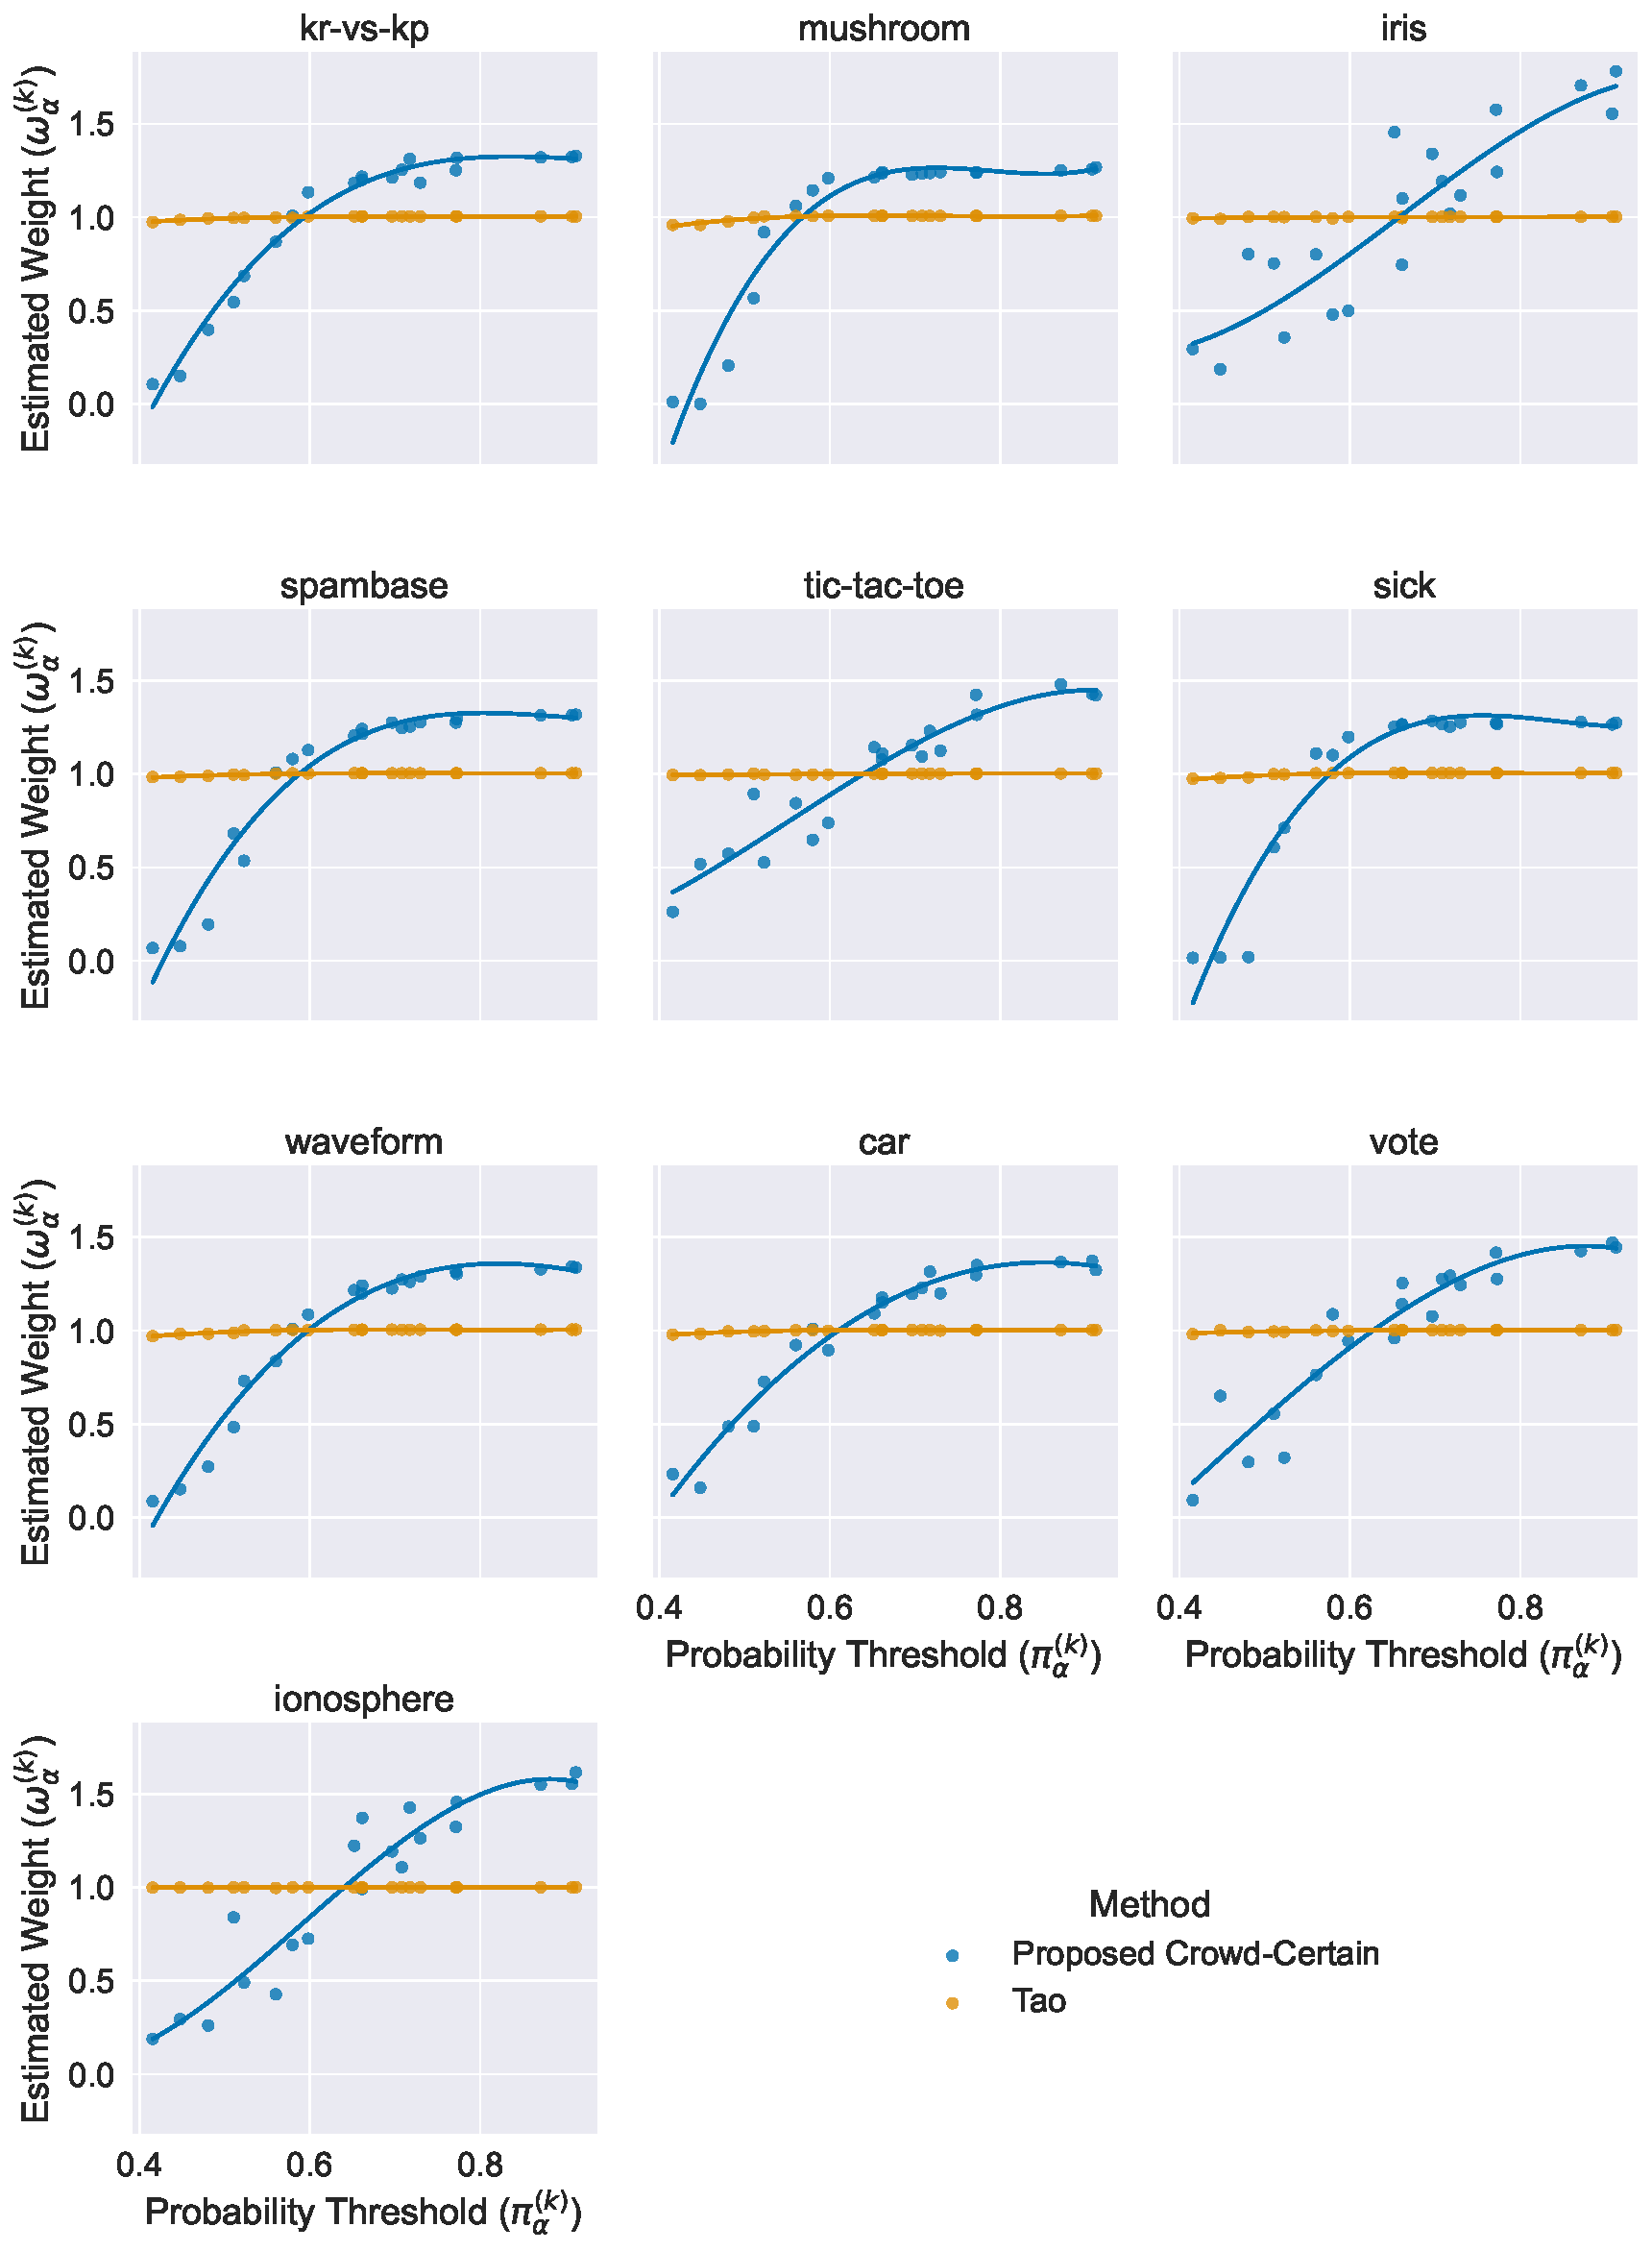
\includegraphics[width=0.9\textwidth]{\figurepath{lmplot_weight_strength_relation/lmplot_weight_strength_relation.pdf}}
    \caption{Comparison of weight computation techniques across ten different datasets. Each subplot corresponds to a unique dataset, illustrating the relationship between the randomly assigned annotator's probability threshold ($\pi_\alpha^{(k)}$) (horizontal axis) and the computed weights ($\omega_{\alpha}^{(k)}$) (vertical axis) for the proposed aggregation technique with penalization ``crowd-certain'' and Tao~\cite{tao_Label_2020}. The individual data points represent actual measured weights, while the curve stands for the regression line.}%
    \label{fig:crowd.Fig.1.weight}
\end{figure}

\subsection{Accuracy}
The Figure~\ref{fig:crowd.accuracy_per_worker} portrays a thorough accuracy comparison of our novel label aggregation technique, termed ``Crowd-Certain'', against ten existing methods, evaluated over ten distinct datasets. Each dataset was labeled by three different workers, with labels generated based on a uniform distribution and specific probability thresholds $\Pi_\alpha$ as explained in Section~\ref{subsec:methods.generating_fictitious_labelset}.

For a comprehensive evaluation, all experiments were repeated three times using different random seed numbers to account for randomness. The accuracy scores presented in the figure represent the average of these three runs and illustrate the degree of concordance between the aggregated label $\nu^{(i,k)}$ from each technique and the actual ground truth $y^{(i,k)}$.

It is important to note that, in the execution of our proposed technique, ``Crowd-Certain'', the aggregated labels were derived through the application of the predicted probabilities, denoted as $\eta_{\alpha}^{(i,k)}$. This approach is significant as it enables the reuse of trained classifiers on future sample data, eliminating the need for recurrent simulation processes - a substantial advantage in terms of computational efficiency. Conversely, the methodologies of existing techniques necessitated the use of actual crowd labels $z_\alpha^{(i,k)}$ to determine the aggregated labels. For example, in case of Tao~\cite{tao_Label_2020} the aggregated labels were obtained using the equation~\ref{eq:crowd.Eq.12.aggregated-label_for_benchmarks}. These methods inherently involve re-running simulations for every new dataset, which could be computationally expensive and time-consuming.
%
\begin{equation}
    \nu^{(i,k)} =
    \begin{cases}
        1 & \text{if } \left(\sum_{\alpha=1}^{M} \omega_{\alpha}^{(k)}\, z_{\alpha}^{(i,k)}\right) > 0.5 \\
        0 & \text{otherwise}
    \end{cases}
    \quad \forall i, k
    \label{eq:crowd.Eq.12.aggregated-label_for_benchmarks}
\end{equation}
%
Across all ten datasets, it is clear that the "Crowd-Certain" method consistently outperforms the existing methods, yielding higher average accuracy rates. For example, in the 'kr-vs-kp' dataset, our proposed "Crowd-Certain" method achieved an average accuracy of approximately 0.923, significantly exceeding the highest-performing existing method that reached an accuracy of about 0.784. This trend holds true across other datasets as well, such as 'mushroom', 'spambase', and 'tic-tac-toe', where the "Crowd-Certain" method achieves superior average accuracies of around 0.980, 0.900, and 0.741, respectively. In contrast, the competing methods struggled to exceed an average accuracy of 0.771 in these datasets.
%
\begin{figure*}[htbp]
\centering
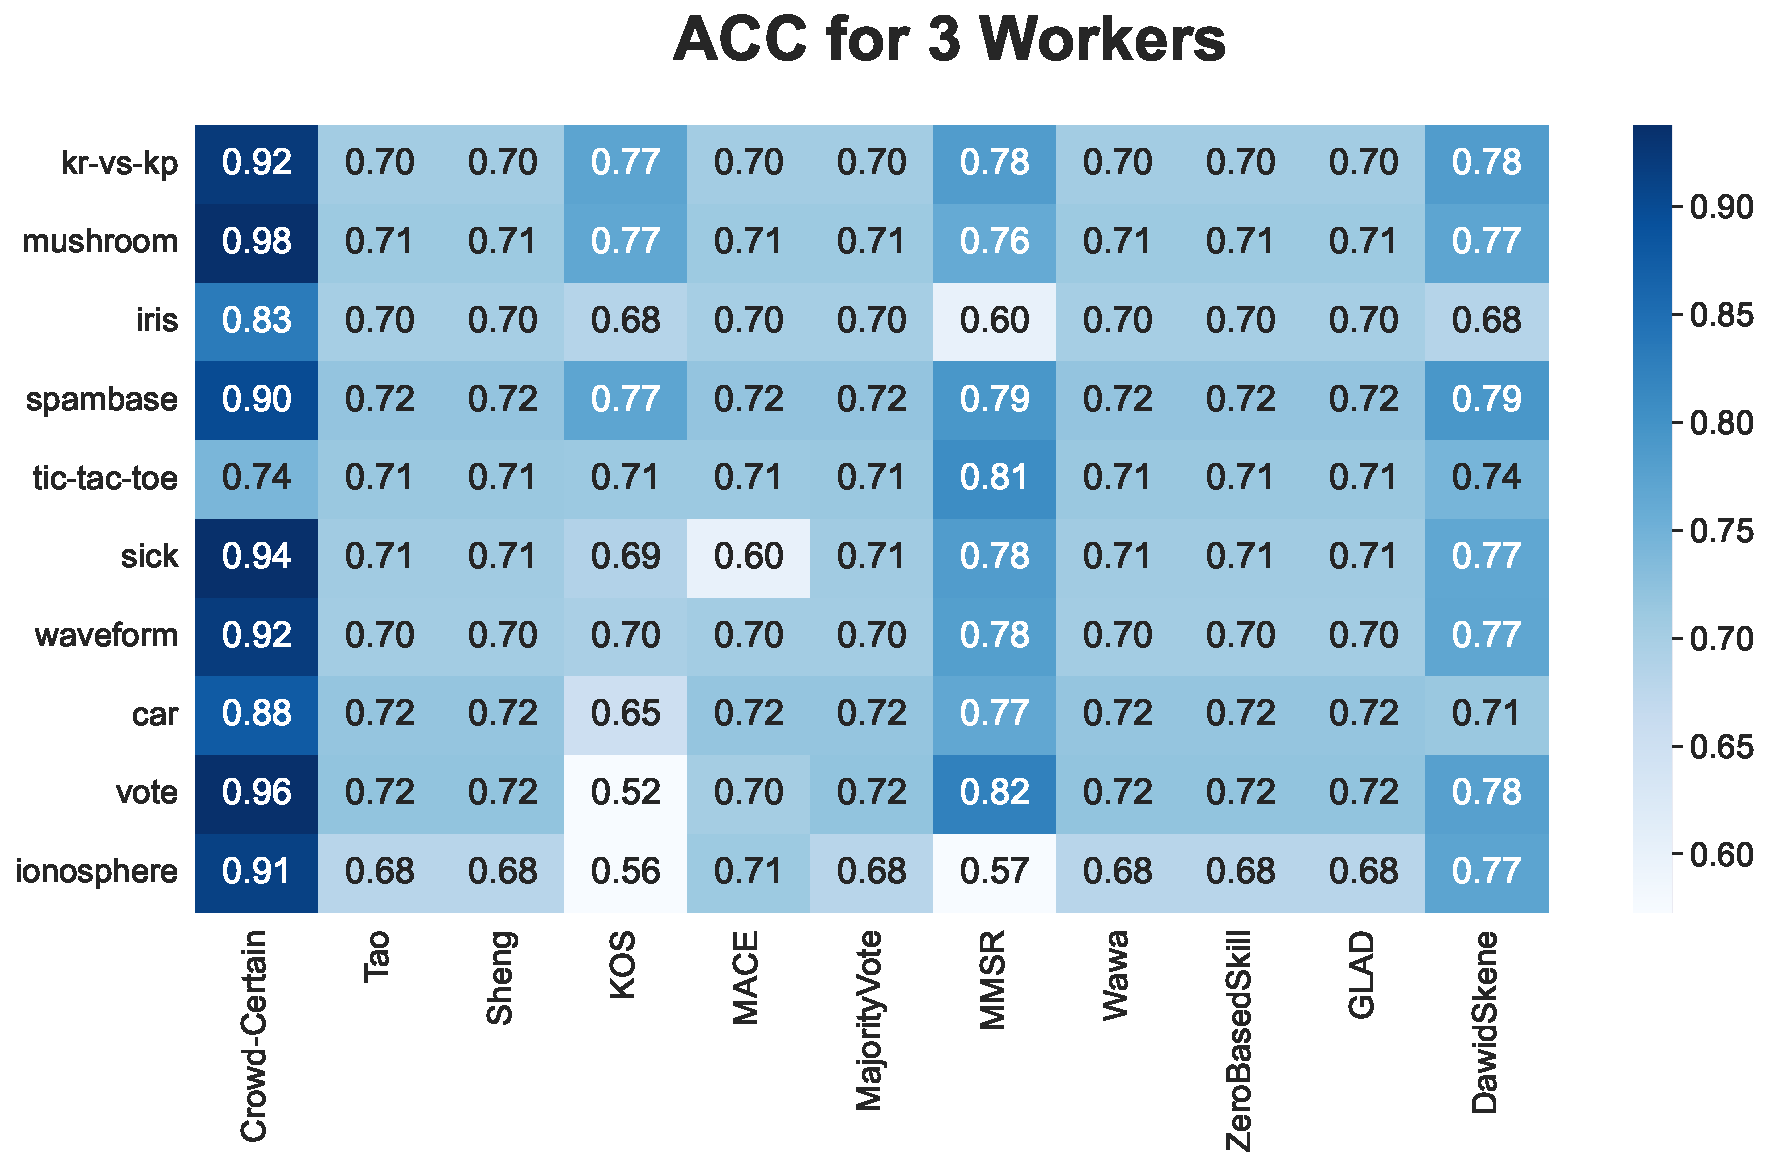
\includegraphics[width=0.9\textwidth]{\figurepath{figure_metrics_mean_over_seeds_per_dataset_per_worker_ACC/figure_metrics_mean_over_seeds_per_dataset_per_worker_ACC.pdf}}
\caption{Comparison of Accuracy Scores for Multiple Label Aggregation Techniques on Various Datasets. The figure displays the mean accuracy score obtained across three independent trials for the proposed method ("Crowd-Certain") and ten existing label aggregation techniques. The trials were conducted using three labelers (workers) per dataset. The aggregated labels for "Crowd-Certain" were derived using predicted probabilities, allowing for reuse of trained classifiers. In contrast, existing techniques used actual crowd labels, necessitating repeated simulations.}%
\label{fig:crowd.accuracy_per_worker}
\end{figure*}

We further extended our experiment to explore the effects of varying the number of annotators, ranging from 3 up to 7. The results shown in Figure~\ref{fig:crowd.Fig.accuracy_all_datasets_workers}, are presented as a series of box plots, each illustrating the distribution of accuracy (1st column), F1 (2nd column), and AUC (3rd column) scores across the 10 datasets for a given number of annotators. These plots provide a clear visual summary of our technique's robust performance across various settings, including the median, quartiles, and potential outliers in the distribution of accuracies. Notably, our proposed "Crowd-Certain" technique consistently shows improvements over the 10 benchmark methods across all scenarios. This enhancement is evident irrespective of the number of annotators involved, further highlighting the robustness and adaptability of the "Crowd-Certain" approach.
\begin{figure*}[htbp]
\centering
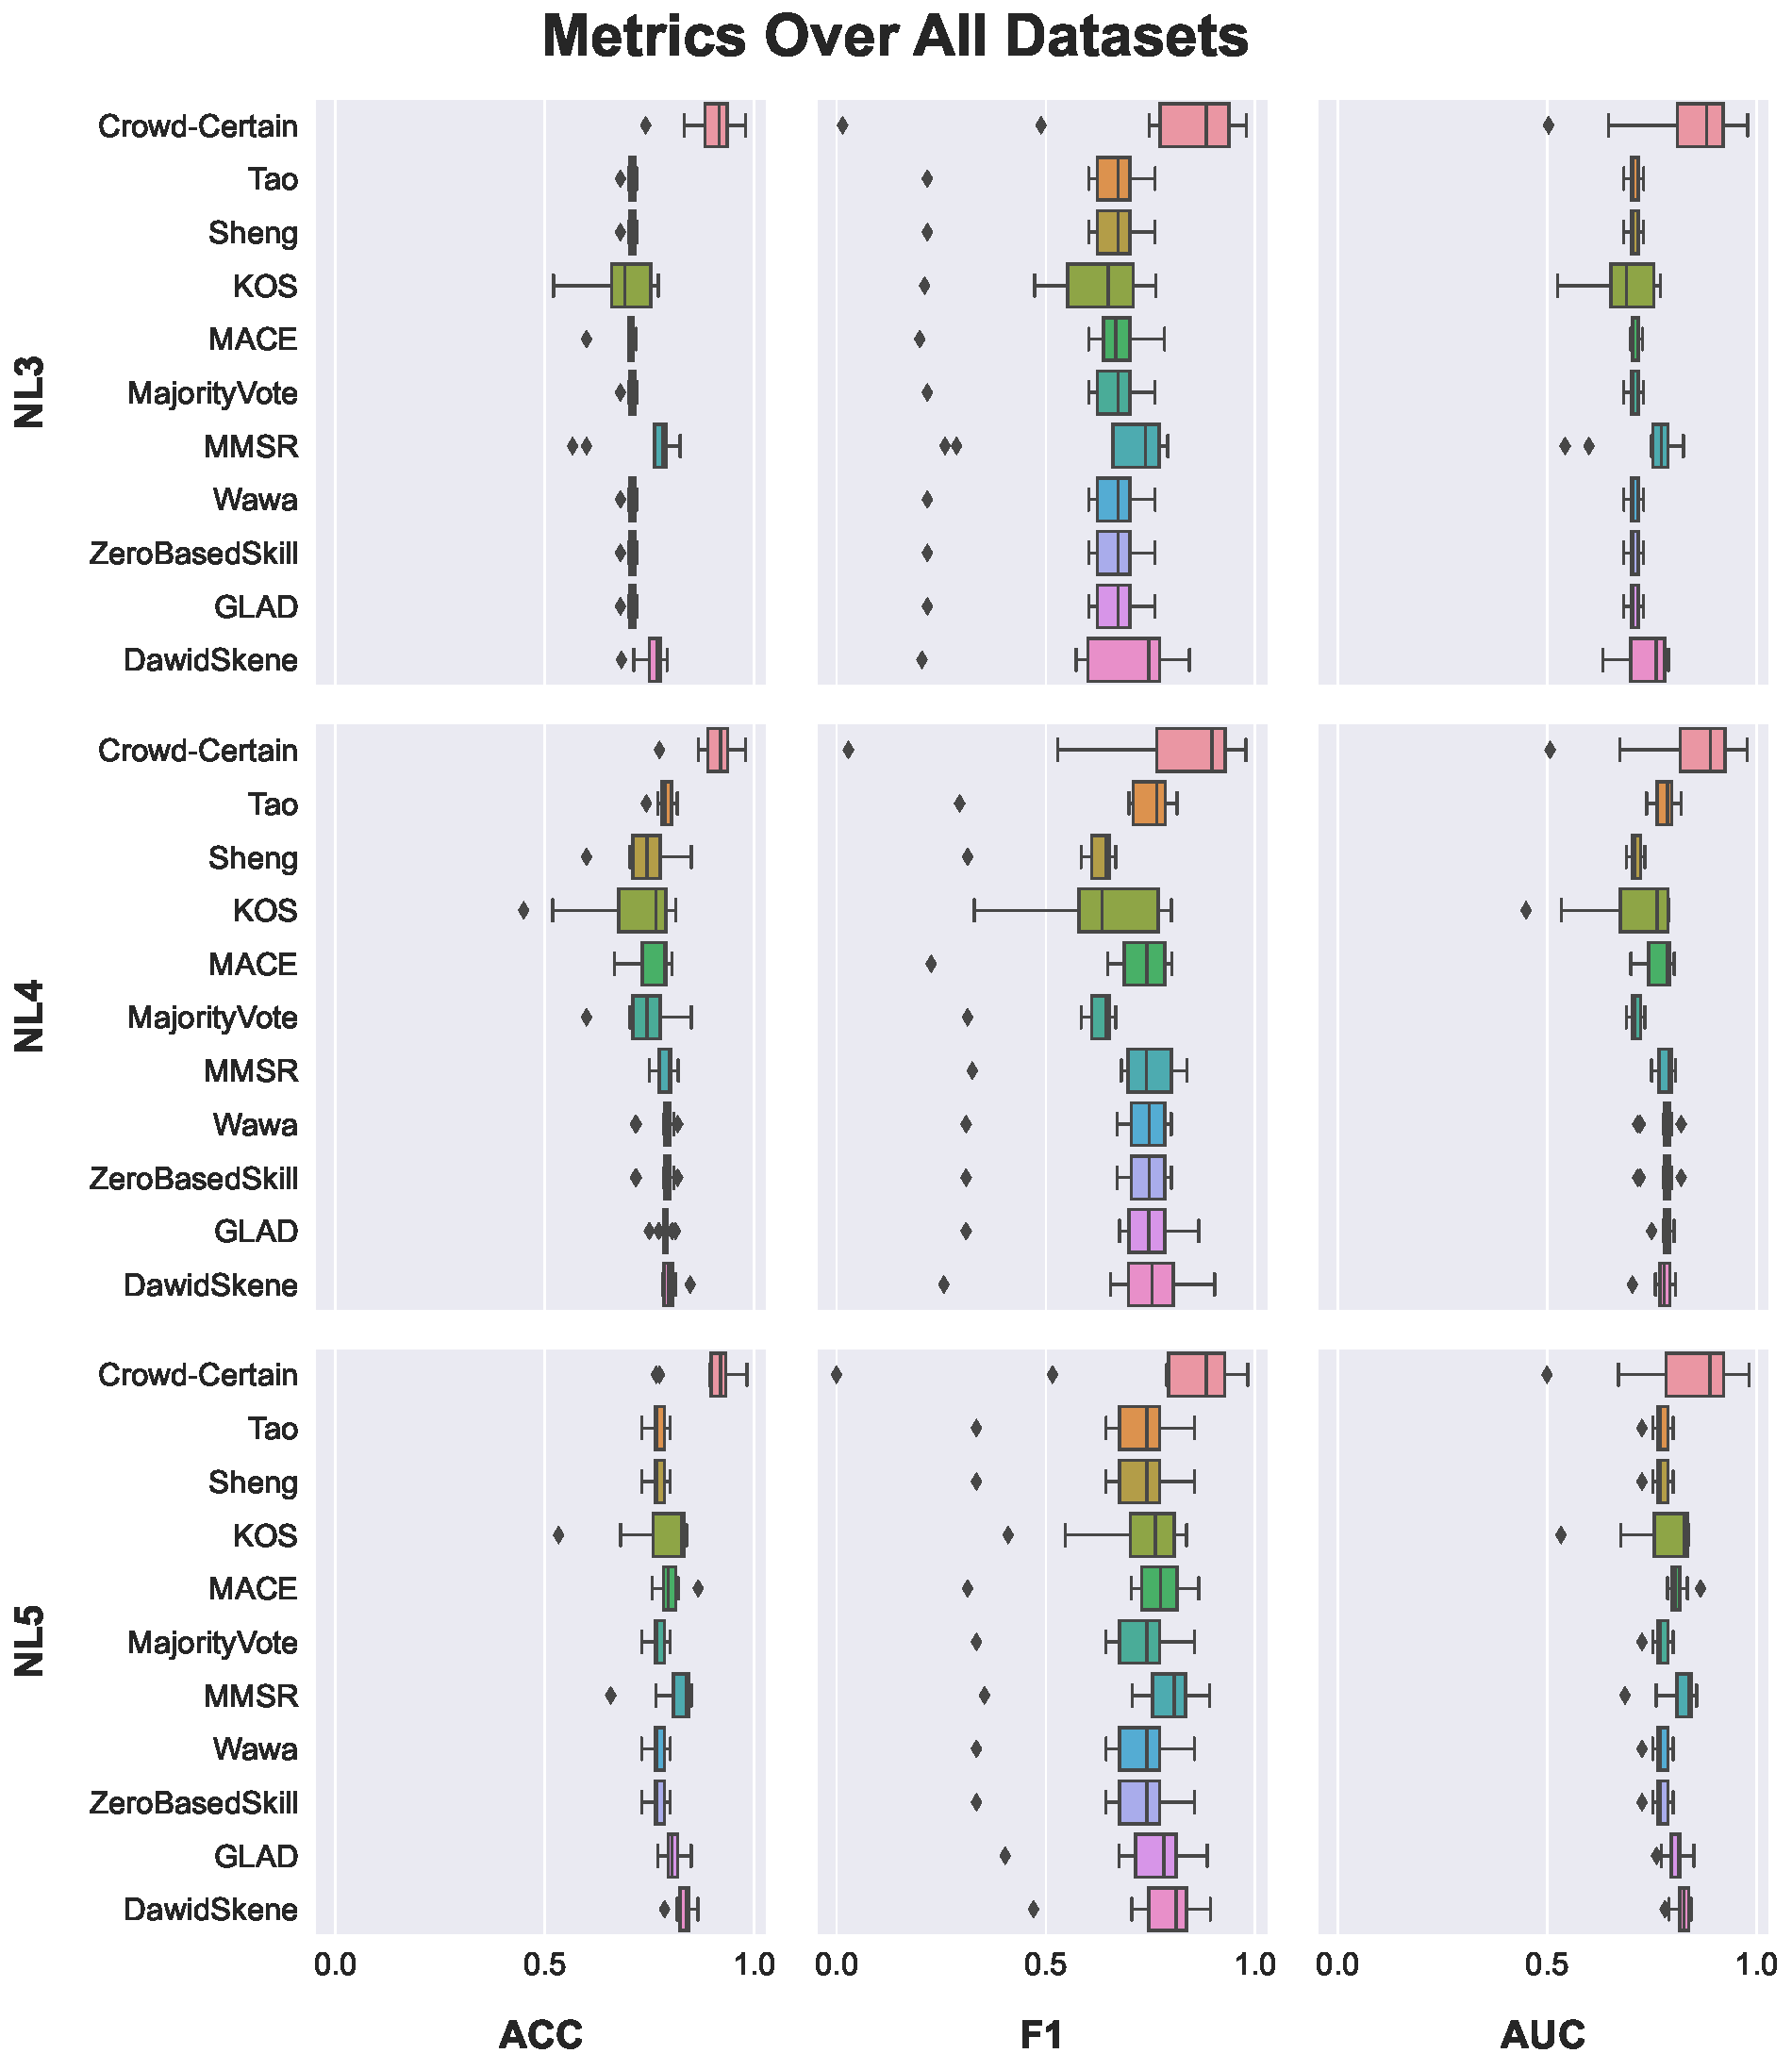
\includegraphics[width=0.9\textwidth]{\figurepath{figure_metrics_all_datasets_workers/figure_metrics_all_datasets_workers.pdf}}
\caption{}%
\label{fig:crowd.Fig.accuracy_all_datasets_workers}
\end{figure*}

\subsection{Confidence Score}
% Figure~\ref{fig:crowd.Fig.2.confidence_scores} present a box plot of the average accuracy for different numbers of annotators, ranging from three to ten. It illustrates the average accuracy of the crowd-certain technique with penalization for both the ``freq” and ``Beta” confidence measurement approaches showing comparable accuracy.
% %
% Figure~\ref{fig:crowd.Fig.4.confidence_score.freq} displays the average accuracy using the ``freq’’ confidence measurement strategy for the proposed crowd-certain technique with and without penalization. The penalization method penalizes annotators for inaccurate labeling before measuring their weights, as demonstrated in Equation~(\ref{eq:crowd.eq.10.consistency-penalized}). The penalized version of the proposed technique shows an improvement in average accuracy and a reduction in variance.

\begin{figure*}[htbp]
\centering
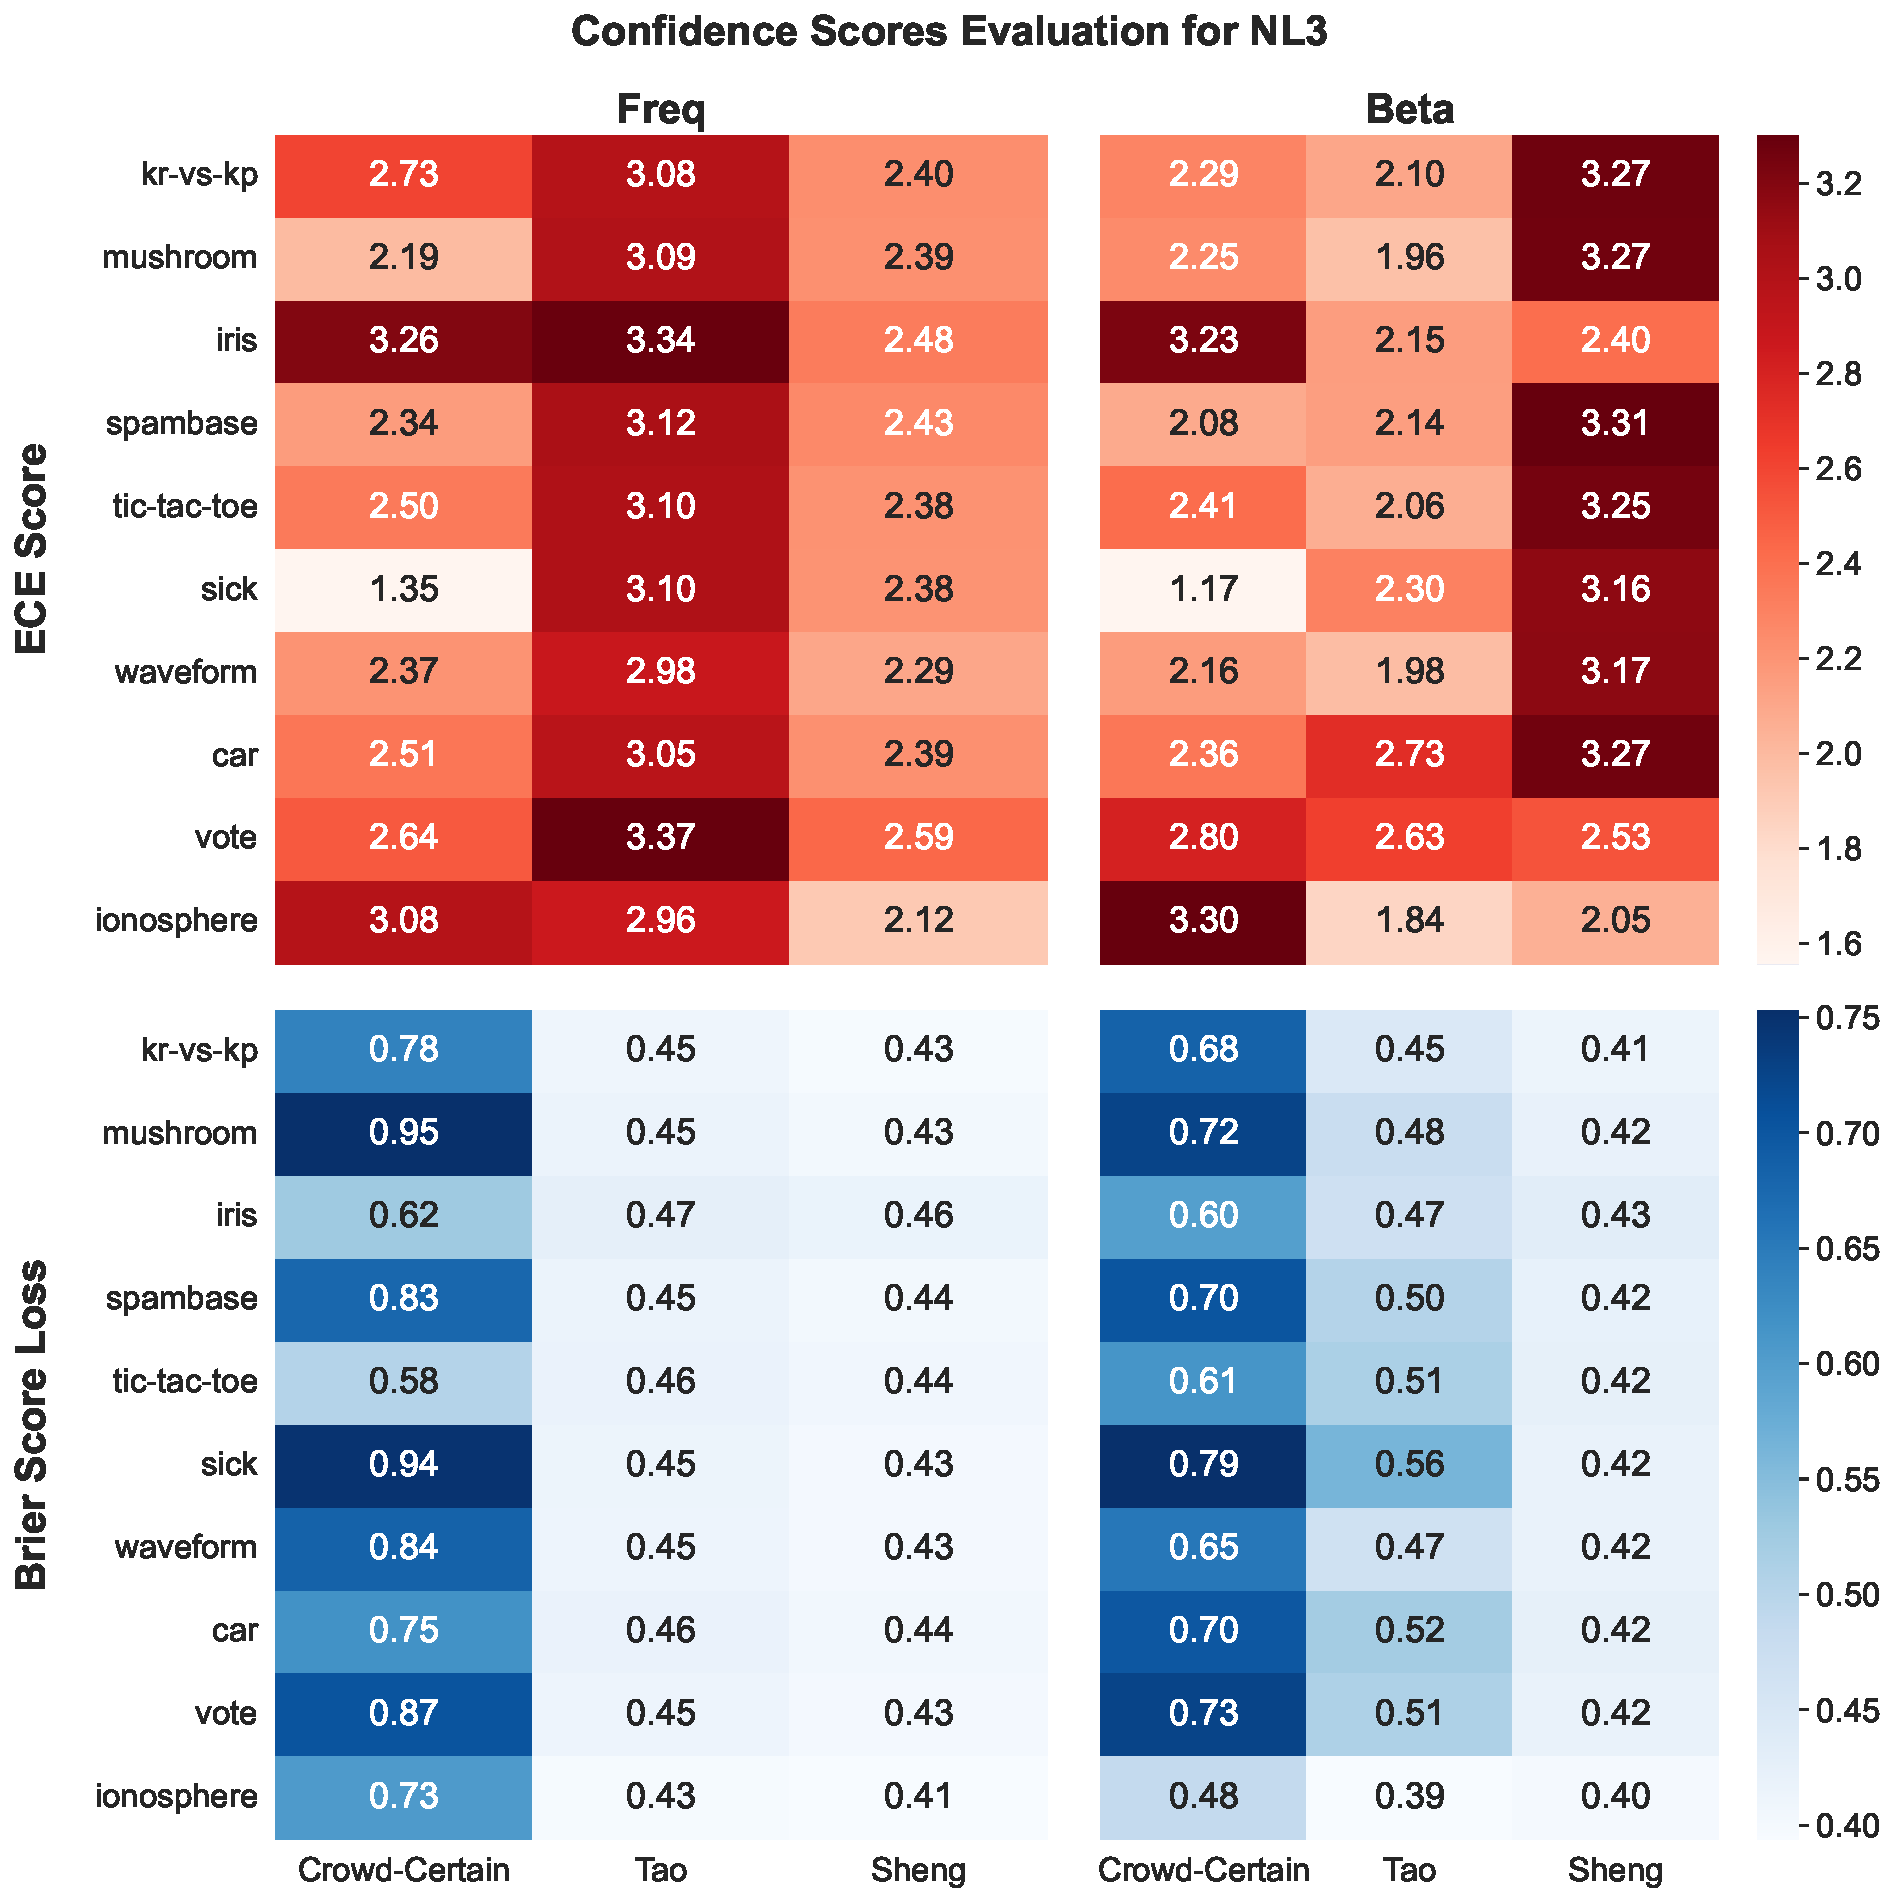
\includegraphics[width=0.9\textwidth]{\figurepath{heatmap_F_evals_all_datasets_NL3/heatmap_F_evals_all_datasets_NL3.pdf}}
\caption{}%
\label{fig:crowd.Fig.confidence_scores_all_datasets_3_workers}
\end{figure*}
%
\begin{figure*}[htbp]
    \centering
    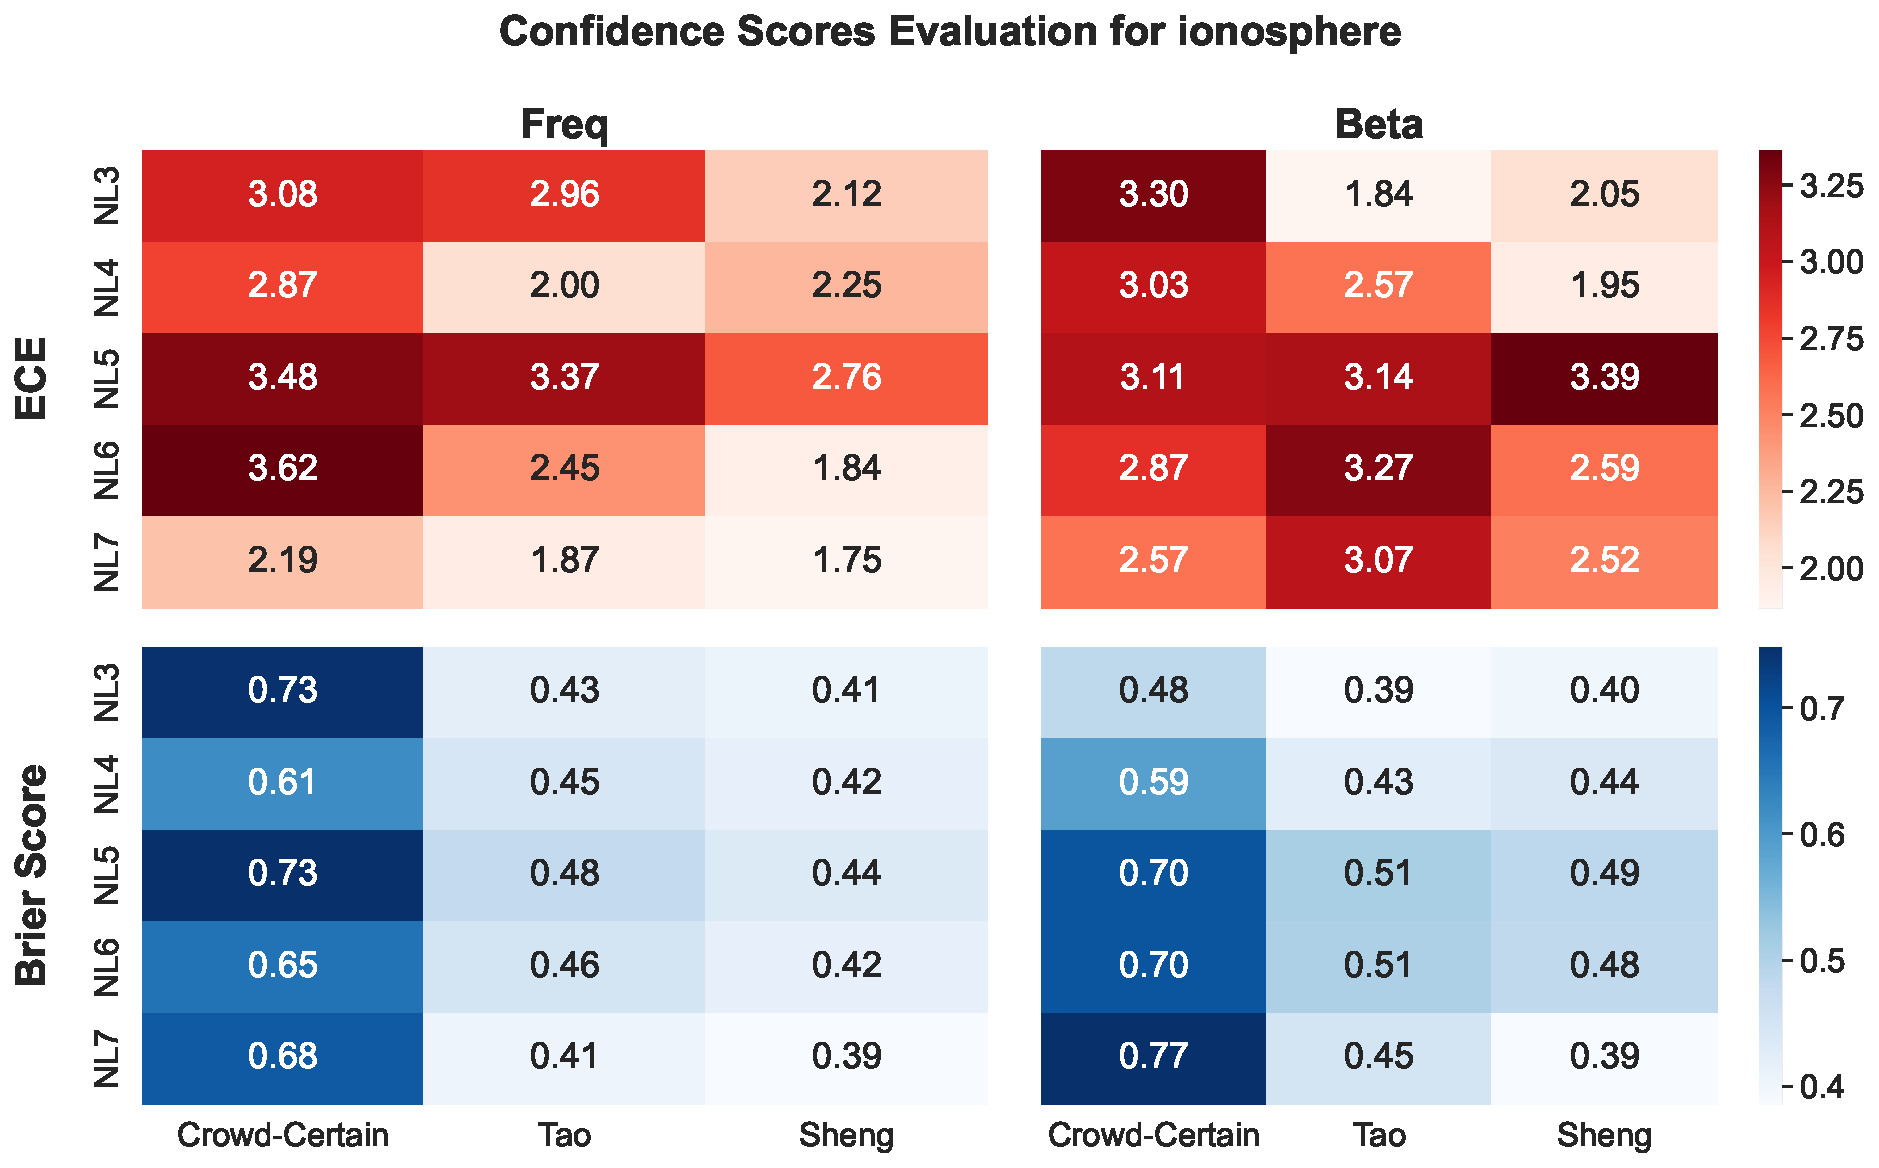
\includegraphics[width=0.9\textwidth]{\figurepath{heatmap_F_evals_ionosphere_all_labelers/heatmap_F_evals_ionosphere_all_labelers.pdf}}
    \caption{}%
    \label{fig:crowd.Fig.confidence_score_ionosphere_all_workers}
\end{figure*}
% Figure~\ref{fig:crowd.Fig.5.confidencescore-beta} shows the average accuracy distribution (``freq'' strategy) of the proposed penalized versus Tao and Sheng for a different number of annotators using the kernel density estimation technique. This demonstrates that the proposed technique outperforms both Tao and Sheng on nine of the ten datasets, with higher average accuracy and less fluctuation over different annotator counts. Table~\ref{tab:crowd.Table.2.crowdcertain_vs_Tao.freq}  shows the statistical data measured between the proposed penalized technique and Tao's method. As can be seen from these results, the proposed technique has a significant improvement for the seven datasets, while delivering similar results for the other three datasets.

% \begin{table}[]
%     \caption{{Statistical tests between the proposed-penalized technique and Tao\unskip~\protect\cite{tao_Label_2020} for the ``freq” confidence measurement strategy.} }
%     \resizebox{\textwidth}{!}{
%     % \scalebox{0.75}{
%         \begin{tabular}{lccclllccrc}
%         \hline
%         \textbf{\begin{tabular}[c]{@{}l@{}}Independent   \\ t-test\end{tabular}} &
%         \textbf{Diff} &
%         \textbf{\begin{tabular}[c]{@{}l@{}}Degrees of \\ freedom\end{tabular}} &
%         \textbf{t} &
%         \textbf{\begin{tabular}[c]{@{}l@{}}2-sided \\ p-value\end{tabular}} &
%         \textbf{\begin{tabular}[c]{@{}l@{}}Diff\textless{}0 \\ p-value\end{tabular}} &
%         \textbf{\begin{tabular}[c]{@{}l@{}}Diff\textgreater{}0 \\ p-value\end{tabular}} &
%         \textbf{Cohen d} &
%         \textbf{Hedge's g} &
%         \textbf{\begin{tabular}[c]{@{}l@{}}Glass's \\ delta\end{tabular}} &
%         \textbf{Pearson r} \\ \hline
%             Kr-vs-kp    & -0.044 & 12 & -6.171 & 0     & 0     & 1     & -3.299 & -3.088 & -2.743 & 0.872 \\
%             mushroom    & -0.012 & 12 & -2.781 & 0.017 & 0.008 & 0.992 & -1.487 & -1.392 & -1.076 & 0.626 \\
%             iris        & -0.012 & 12 & -0.506 & 0.622 & 0.311 & 0.689 & -0.271 & -0.253 & -0.226 & 0.145 \\
%             spambase    & -0.031 & 12 & -3.691 & 0.003 & 0.002 & 0.998 & -1.973 & -1.847 & -1.458 & 0.729 \\
%             tic-tac-toe & -0.036 & 12 & -4.612 & 0.001 & 0     & 1     & -2.466 & -2.308 & -2.156 & 0.8   \\
%             sick        & 0.002  & 12 & 0.294  & 0.774 & 0.613 & 0.387 & 0.157  & 0.147  & 0.112  & 0.085 \\
%             waveform    & -0.025 & 12 & -5.118 & 0     & 0     & 1     & -2.736 & -2.561 & -2.022 & 0.828 \\
%             car         & -0.008 & 12 & -0.779 & 0.451 & 0.226 & 0.774 & -0.416 & -0.39  & -0.309 & 0.219 \\
%             vote        & -0.033 & 12 & -5.352 & 0     & 0     & 1     & -2.861 & -2.678 & -2.112 & 0.84  \\
%             ionosphere  & -0.061 & 12 & -6.047 & 0     & 0     & 1     & -3.232 & -3.026 & -2.586 & 0.868 \\ \hline
%         \end{tabular}}%
%     \label{tab:crowd.Table.2.crowdcertain_vs_Tao.freq}
% \end{table}

\section{Discussion}\label{sec:crowd.discussion}
Label aggregation is a critical component of crowdsourcing and ensemble learning strategies. Many generic label aggregation algorithms fall short because they do not account for the varying reliability of the annotators. In response to this, we have developed a novel label aggregation method that calculates a reliability score for each annotator based on the annotator’s consistency versus a trained classifier. In the first approach (proposed techniques without penalization), we utilize uncertainty estimates to assign each annotator a more accurate weight, which correlates with their agreement with others and their consistency during labeling. In the second approach (proposed technique with penalization. Also noted as crowd-certain), we improve  on this technique by penalizing the annotator for their disagreements with other annotators (shown in Eq.~\ref{eq:crowd.eq.10.consistency-penalized} and hence mitigate the effect of annotators’ bias when calculating the final weights $\omega_{\alpha}^{(k)}$).
The first part (calculating weights based on annotator’s consistency) of the proposed crowd-certain algorithm (the proposed technique with penalization) is essential because non-expert annotators often exhibit more irregular consistency during labeling than experts, as they are not well trained to identify specific features. This (utilizing consistency when assigning weights to each annotator) helps to differentiate expert and non-expert annotators. The goal of the second part (penalty for voting against the majority) of the algorithm is to prevent the algorithm from assigning disproportionately high weights to annotators who are consistently incorrect. For example, if annotators consistently mislabel a specific bird species, the second part penalizes them for their error, despite their consistency.
Furthermore, our method reports a single weight for the entire dataset instead of individual weights for each instance. This enables the reuse of calculated weights for future unlabeled test samples without needing to reacquire labels or retrain classifiers each time new data need labeling. While we have not assessed our method in multi-label scenarios, the proposed techniques are anticipated to perform comparably on multi-label datasets, considering that all steps of the proposed approach involve per-class calculations. Experiments conducted on various crowdsourcing datasets demonstrate that our proposed methods outperform existing techniques in terms of accuracy and variance, especially when there are few annotators available.

\section{Availability of Data and Materials}
The code can be found in \href{https://github.com/artinmajdi/crowdcertain}{crowd-certain}

\section{Appendices}
\section*{List of abbreviations}
\section*{Competing interests}
\section*{Acknowledgements}
